\documentclass[pdflatex,11pt]{aghdpl}
% \documentclass{aghdpl}               % przy kompilacji programem latex
% \documentclass[pdflatex,en]{aghdpl}  % praca w języku angielskim
\usepackage[polish]{babel}
\usepackage[utf8]{inputenc}

% dodatkowe pakiety
\usepackage{enumerate}
\usepackage{enumitem}
\usepackage{listings}
\usepackage[polish]{algorithm2e}
\usepackage{longtable}
\usepackage{listings}
\usepackage{bm}
\usepackage{amsmath}
\lstloadlanguages{TeX}

\lstset{
  literate={ą}{{\k{a}}}1
           {ć}{{\'c}}1
           {ę}{{\k{e}}}1
           {ó}{{\'o}}1
           {ń}{{\'n}}1
           {ł}{{\l{}}}1
           {ś}{{\'s}}1
           {ź}{{\'z}}1
           {ż}{{\.z}}1
           {Ą}{{\k{A}}}1
           {Ć}{{\'C}}1
           {Ę}{{\k{E}}}1
           {Ó}{{\'O}}1
           {Ń}{{\'N}}1
           {Ł}{{\L{}}}1
           {Ś}{{\'S}}1
           {Ź}{{\'Z}}1
           {Ż}{{\.Z}}1
}

%---------------------------------------------------------------------------

\author{Rafał Studnicki}
\shortauthor{R. Studnicki}

\titlePL{Analiza wybranych deskryptorów cech wykorzystywanych w algorytmach detekcji obiektów
}
\titleEN{Analysis of feature descriptors used in object detection algorithms}

\shorttitlePL{Analiza wybranych deskryptorów cech wykorzystywanych w algorytmach detekcji obiektów} 
\shorttitleEN{Analysis of feature descriptors used in object detection algorithms}

\thesistypePL{Praca inżynierska}
\thesistypeEN{Bachelor of Science Thesis}

\supervisorPL{dr hab. inż. Marek Gorgoń,\\prof. nz. AGH}
\supervisorEN{Marek Gorgoń Ph.D Eng.}

\date{2012}

\departmentPL{Katedra Automatyki i Inżynierii Biomedycznej}
\departmentEN{Department of Automatics and Biomedical Engineering}

\facultyPL{Wydział Elektrotechniki, Automatyki, Informatyki i Inżynierii Biomedycznej}
\facultyEN{Faculty of Electrical Engineering, Automatics, Computer Science and Biomedical Engineering}

\acknowledgements{Miejsce na podziękowania}

\setlength{\cftsecnumwidth}{10mm}

%---------------------------------------------------------------------------

\begin{document}

\titlepages

\tableofcontents
\clearpage

\chapter{Wprowadzenie}
\label{cha:wprowadzenie}

W rozdziale tym zaprezentowano ogólne cele i wyzwania związane z tworzeniem automatycznych systemów wizyjnych oraz przedstawiono znaczenie detekcji obiektów w tychże systemach.
Wymieniono także cele, dla jakich powstała niniejsza praca, a także streszczono jej zawartość na przestrzeni kolejnych rozdziałów. 

%---------------------------------------------------------------------------

\section{Wykorzystanie komputerowych systemów wizyjnych}
\label{sec:systemy}

Dzięki coraz niższym cenom kamer cyfrowych wysokiej rozdzielczości, a także wyższej dostępności komputerów o dużej mocy obliczeniowej, temat budowy komputerowych systemów wizyjnych zyskał w ostatnich czasach dużą popularność. To rosnące powodzenie z kolei, była motywacją do dużego, niespotykanego do tej pory, zainteresowania rozwojem w dziedzinie algorytmów związanych z przetwarzaniem i rozpoznawaniem obrazów. Efektem tego było powstanie, na przestrzeni ostatnich kilkunastu lat, w wielu ośrodkach badawczych na całym świecie, wielu propozycji metod do realizacji konkretnych zadań związanych z automatycznym rozpoznawaniem wizji, z których wiele z nich zostało użytych z~powodzeniem w praktyce.

Wśród dziedzin, którym szybki rozwój systemów wizyjnych przynosi najwięcej korzyści można wymienić m.in.:
\begin{itemize}
\item informatykę\\*
na systemach wizyjnych swą budowę opierają interfejsy multimodalne, rozpoznające np. gesty wykonywane przez operatora;
\item automatykę\\*
systemy wizyjne są podstawą działania robotów potrafiących podejmować decyzje na podstawie danych o świecie zewnętrznym;
\item komunikację\\*
dzięki systemom wizyjnym można pozyskiwać dane o natężeniu ruchu i na jego podstawie np. dynamicznie sterować sygnalizacją świetlną;
\item przemysł samochodowy\\*
systemy wizyjne wykorzystywane są w systemach zwiększających bezpieczeństwo jazdy, np. wykrywające znaki drogowe;
\item systemy monitoringu\\*
systemy wizyjne pozwalają na automatyczne wykrycie podejrzanych zachowań np. na lotnisku.
\end{itemize}

Głównym zadaniem komputerowego systemu wizyjnego jest wyodrębnienie z zadanego obrazu, statycznego bądź ruchomego, pewnej informacji a następnie wykonanie na jej podstawie pewnej czynności, najczęściej specyficznej dla konkretnego systemu.
Zadanie to jest realizowane za pomocą kilku etapów, które mają na celu jak największe upodobnienie działania takiego systemu do ludzkiego widzenia:
\begin{itemize}
\item akwizycji obrazu;
\item przetwarzania wstępnego obrazu;
\item analizy obrazu;
\item rozpoznania obrazu;
\item podjęcia decyzji.
\end{itemize}

W przypadku ludzkiego zmysłu wzroku, którego każdego dnia używamy wielokrotnie we wszystkich czynnościach życiowych, nie mamy nawet świadomości ich istnienia. Dzieje się tak dlatego, że wykonywane są one przez mózg w sposób bardzo szybki i naturalny.
Jednak tworząc sztuczny system wizyjny musimy mieć świadomość złożoności procesu jaki prowadzi do podjęcia decyzji na podstawie obrazu. Dodatkowym jego utrudnieniem niech będzie fakt, że do tej pory sposób, w jaki ludzki mózg dokonuje analizy obrazu otrzymanego od narządu wzroku, nie został dokładnie zbadany.\\*
Oprócz tego, do niedoskonałości sztucznych systemów wizyjnych można zaliczyć m.in.
\begin{itemize}
\item niedoskonałość kamer, np. powstawanie szumów;
\item utratę informacji w trakcie projekcji obrazu trójwymiarowego na dwuwymiarowy;
\item zmiany oświetlenia obserwowanej sceny;
\item częściowe lub całkowite zasłonięcie obiektów na scenie.
\end{itemize}

Na dłuższą metę jednak, użycie komputerowych systemów wizyjnych niesie za sobą wiele korzyści w zastosowaniach, w których zostały one już dobrze sprawdzone i istnieje możliwość zastąpienia nimi ludzkiego zmysłu wzroku.\\*

Należą do nich m.in:
\begin{itemize}
\item eliminacja błędów ludzkich wynikających z takich czynników jak np. stres;
\item możliwość rozpoznawania obrazów poza zakresem światła widzialnego;
\item możliwość umieszczenia systemu w miejscach niedostępnych lub nieopłacalnych dla człowieka;
\item krótki czas reakcji.
\end{itemize}

%---------------------------------------------------------------------------

\section{Znaczenie detekcji obiektów w komputerowych systemach wizyjnych}
\label{sec:detekcjaWSystemach}

Jak wspomniano wyżej, w wielu swoich zastosowaniach systemy wizyjne opierają swoje działanie na detekcji pewnych obiektów na obrazie.
Jest to jednak jeden z najbardziej wymagających problemów widzenia automatycznego, ze względu na to, że na dwuwymiarowym rzucie obiektu na obraz, który dostępny jest do analizy, interesujący nas obiekt zmienia swój kształt w czasie, staje się on częściowo przysłonięty czy zmienia się poziom jego oświetlenia.
W wielu przypadkach sama detekcja obiektu na obrazie jest tylko jednym z elementów działania odpowiedniego systemu wizyjnego. Na przykład w~przypadku systemu, którego zadaniem jest analiza sposobu chodu człowieka, analiza taka dokonywana jest dopiero po wcześniejszym wykryciu obecności człowieka w zadanej strefie przez odpowiedni system detekcji.
Do innych zastosowań takich systemów zaliczają się np.: detekcja przechodniów~w~inteligentnych systemach prowadzenia pojazdów czy detekcja obiektów znajdujących się w zabronionej strefie (np. osoby niepożądanej na terenie prywatnym czy pozostawionej walizki na lotnisku).

Jak łatwo zauważyć, rozpoznanie konkretnych obiektów ma szerokie zastosowanie np. w systemach monitoringu, gdzie omyłkowe podniesienie alarmu w~sytuacji potencjalnego zagrożenia może mieć znaczne konsekwencje. Dlatego też, niejednokrotnie, starając się opracować metodę wykrywającą pewną klasę obiektów na obrazie, poza osiągnięciem jak najlepszej trafności metody, szczególnie dużą uwagę poświęca się maksymalnie możliwemu wyeliminowaniu odsetku niepoprawnych detekcji.

Dodatkowym wyzwaniem dla autorów metod detekcji obiektów jest fakt, że nie istnieje rozwiązanie sprawdzające się tak samo dobrze dla każdej klasy poszukiwanych obiektów. Wynika to z faktu istnienia różnych deskryptorów dla różnych klas obiektów, a także różnych metod klasyfikacji, dzięki którym można w dobrym stopniu odróżnić obiekt należący do danej klasy od obiektu, który do niej nie należy (w przypadku detekcji człowieka może to być np. pewien sposób opisu sylwetki jego ciała, podczas gdy inny rodzaj obiektu będzie wykrywany w dużo lepszym stopniu wykorzystując informację o kolorze). Dlatego też, w momencie budowy systemu wizyjnego przeznaczonego do detekcji konkretnej klasy obiektów, jego autorzy często zmuszeni są do przeprowadzenia szeregu badań w celu wybrania jak najlepszych deskryptorów dla danego problemu i wprowadzenia potencjalnych ulepszeń do istniejących już metod tak, aby w ich konkretnym zastosowaniu sprawdzały się jak najlepiej.

%---------------------------------------------------------------------------

\section{Rola deskryptorów cech w rozpoznawaniu obrazów}
\label{sec:deskryptory}

Obliczenie deskryptora cech polega na pewnym zmniejszeniu wymiarów potrzebnych do opisu pewnego zjawiska. Dobrze zbudowany deskryptor cech powinien działać w taki sposób, aby w procesie redukcji ilości informacji pomijać np. dane, których obecność powielona jest w kilku miejscach wejścia, ale przede wszystkim pomijać te dane, które są bezużyteczne w kontekście danego problemu. Dobry deskryptor cech powinien także dodatkowo eksponować te informacje, które są najważniejsze dla danego problemu, tak aby, mając do dyspozycji tylko i wyłącznie wynik jego działania, można było w nieskomplikowany sposób stwierdzić jakich danych wejściowych użyto do jego obliczenia.

Głównym powodem użycia deskryptorów cech jest zdecydowanie mniejsza złożoność czasowa~i pamięciowa potrzebna do ich przetworzenia przez klasyfikator. Ma to szczególne znaczenie w przypadku zadania rozpoznawania obrazów, gdzie na wejściu zazwyczaj otrzymuje się obraz, często w wysokiej rozdzielczości. W takim wypadku analiza "piksel po pikselu" jest zbyt wymagająca czasowo, by można jej użyć w rzeczywistych systemach rozpoznawania obrazów. W celu poradzenia sobie z tym problemem, szuka się odpowiednich deskryptorów cech, które w dobry sposób zawierają w sobie informacje z obrazu wejściowego ważne w kontekście zadania konkretnego systemu wizyjnego.

%---------------------------------------------------------------------------

\section{Cele pracy}
\label{sec:celePracy}

Celem niniejszej pracy jest bezpośrednie porównanie wybranych deskryptorów cech używanych w~metodach detekcji obiektów na obrazie cyfrowym. Zbadanie działania deskryptorów na dokładnie tym samym zestawie obrazów testowych i używając tego samego sposobu dokonywania klasyfikacji pozwoli w sposób wiarygodny porównać deskryptory pod względem jakościowym w zależności od charakterystyki klasy poszukiwanych obiektów, a także pod względem złożoności czasowej i pamięciowej. Dodatkowym celem pracy jest próba połączenia kilku z wybranych deskryptorów w jeden bardziej złożony i odpowiedź na pytanie czy można uzyskać rozsądną poprawę skuteczności detekcji obiektu konkretnej klasy na obrazie.


%---------------------------------------------------------------------------

\section{Zawartość pracy}
\label{sec:zawartoscPracy}

W rozdziale~\ref{cha:prace} przedstawiono przegląd prac naukowych związanych z automatyczną detekcją obiektów na obrazie, ze szczególnym uwzględnieniem metod wykorzystujących deskryptory cech. W rozdziale~\ref{cha:metodologia} zaprezentowano użyte w testach zestawy obrazów, metodologię przeprowadzonych testów, sposób implementacji środowiska testowego, a także sposoby zbierania wyników do dalszej analizy.\\*
W rozdziale~\ref{cha:deskryptory} opisano, w sposób szczegółowy, zasady działania wybranych metod, sposób ich implementacji, a także zestawiono i przeanalizowano wyniki testów, jakim zostały poddane.\\*
W rozdziale~\ref{cha:laczenie} zaprezentowano propozycje połączenia wybranych deskryptorów, analizując potencjalne korzyści jakie może nieść dane połączenie. Dodatkowo przeanalizowano i opisano wyniki testów, jakim zostały poddane kombinacje deskryptorów.\\*
W rozdziale~\ref{cha:wnioski} podsumowano testy przeprowadzone w rozdziałach~\ref{cha:deskryptory}~i~\ref{cha:laczenie} i wyciągnięto wnioski na temat potencjalnych zastosowań przeanalizowanych metod.
\chapter{Wykorzystanie deskryptorów cech w zadaniach detekcji obiektów}
\label{cha:prace}

W rozdziale tym przedstawiono przegląd literatury dotyczący wybranych metod detekcji obiektów na obrazie opierające się na deskryptorach cech, a także prace związane z ich łączeniem w celu poprawy skuteczności deskryptora.

%---------------------------------------------------------------------------
\section{Proste deskryptory}
\label{sec:prosteDeskryptory}

\subsection{HOG}
Metoda Edge Orientation Histogram (Histogram Orientacji Krawędzi), zaprezentowana po raz pierwszy w pracy \cite{Freeman94} oraz Scale-Invariant Feature Transform (SIFT - Skalo-niezmiennicze przekształcenie cech), przedstawiona w pracy \cite{Lowe04}, stały się inspiracją dla stworzenia metody, którą zaproponowali Navneet Dalal i Bill Triggs w \cite{Dalal05}, której główną ideą jest budowa lokalnych histogramów orientacji krawędzi na przestrzeni całego obrazu. Autorom udało się pokazać, że obecność obiektu i jego kształt można w dobry sposób opisać poprzez lokalny rozkład wartości gradientu i jego orientacji bez znajomości dokładnego położenia krawędzi.

Obraz wejściowy dzielony jest na bloki, które zostają z kolei podzielone na komórki.
Deskryptor HOG wyliczany jest na podstawie długości i orientacji gradientu wyliczonego na obrazie wejściowym. W każdej komórce budowany jest histogram, w którym cechą jest kąt nachylenia gradientu, a liczebnością suma jego długości. W celu redukcji zjawiska aliasingu, krokiem poprzedzającym dodanie wartości do histogramu powinna być interpolacja, zarówno pomiędzy histogramami w sąsiadujących ze sobą komórkach jak i pomiędzy kątami. Kolejnym ważnym krokiem zaproponowanej metody jest normalizacja histogramów w obrębie bloków. Jest to spowodowane faktem, że w różnych częściach obrazu może się on różnić jasnością, co z kolei skutkuje większy kontrast między tłem a obiektami pierwszego planu, co wpływa na wartość wyliczonego gradientu.
Ostatecznie, deskryptor dla obrazu wejściowego reprezentowany jest przez połączenie histogramów na przestrzeni całego obrazu.

Aby jednak możliwe było wykrycie obiektu na realnym obrazie, np. pochodzącym z kamery, autorzy stosują metodologię tzw. ruchomego okna, polegającą na podzielenia obrazu na fragmenty obrazu zgodne co do rozmiaru z obrazami treningowymi i dokonania próby detekcji na podstawie deskryptora wyliczonego właśnie w każdym z tych fragmentów.

Dodatkowo, zaproponowane podejście, polegające na niedokładnym odwzorowaniu przestrzeni w deskryptorze (użycie stosunkowo dużych bloków i komórek jako lokalnej reprezentacji obszaru obrazu) i stosunkowo dokładnego odwzorowania kąta nachylenia krawędzi, pozwala na wiarygodną reprezentację obiektów, takich jak sylwetki ludzkie. Wynika to z faktu, że przemieszczenie ciała na obrazie wpływa na zmianę wartości deskryptora w nieznacznym stopniu. Ponadto, aby możliwe było wykrycie obiektu, który na obrazie wejściowym ma inną skalę niż obiekt na obrazie treningowym, konieczne jest także jego kilkukrotne przeskalowanie obrazu wejściowego, a wynik każdego skalowania poddany jest osobnej detekcji tak, jakby był zupełnie niezależnym obrazem wejściowym.

Efektem badań była nowa metoda detekcji obiektów, która bardzo dobrze sprawdzała się w przypadku detekcji ludzi na obrazie w momencie publikacji, tj. w roku 2005, pozwalała na uzyskanie najlepszych wyników z dostępnych w tym czasie metod, przy założeniu że człowiek na obrazie jest wcale lub w niedużym stopniu przysłonięty przez inne obiekty.

Poza nową metodą, dającą bardzo dobre wyniki w detekcji ludzi na obrazie, osiągnięciem związanym z pracą nad \cite{Dalal05} była budowa nowej bazy obrazów ludzi. Baza ta zawiera zbiór 1805 obrazów ludzi, na zróżnicowanym tle i w różnych pozycjach. Dodatkowo, zdjęcia te są niepozowane, co oznacza że ludzie na nich się znajdujący przyjmują szereg naturalnych pozycji ciała. Baza ta jest dostępna pod adresem \cite{INRIA_set}.

Pod względem zróżnicowania baza ta przewyższała dotychczas przygotowane i została później użyta w~wielu badaniach dotyczących detekcji ludzi na obrazie.

%---------------------------------------------------------------------------
\subsection{Kowariancja cech}
Deskryptor wykorzystujący do opisu cech inne podejście statystyczne niż histogram został zaprezentowany przez O. Tuzel i in. w pracy \cite{Tuzel06}, polegający na użyciu macierzy kowariancji jako deskryptora cech. Podobnie jednak jak w przypadku metody HOG do opisu pewnego obszaru obrazu używany jest histogram, tak w tej metodzie macierz kowariancji również używana jest jako lokalny deskryptor. Metoda ta z powodzeniem została użyta np. w detekcji ludzi na obrazie, czy do rozpoznania tekstur.

Założeniem metody jest użycie wielu informacji, jakie można wydobyć z obrazu, takich jak wartość piksela czy gradient, przy jednoczesnej redukcji liczby wymiarów jakie są potrzebne do ich zapisania. Metoda polega na ekstrakcji, dla każdego piksela obrazu wejściowego, odpowiadającego mu zestawu kilku cech. Mogą to być np. m.in.: pozycja w poziomie, pozycja w pionie, jasność w skali szarości lub w składowych barwnych, wartość gradientu w każdym z kierunków i wypadkowy kąt nachylenia gradientu.
Tak jak w przypadku HOG, ponieważ macierz kowariancji opisuje lokalny fragment obrazu, konieczne jest podzielenie obrazu wejściowego na bloki o odpowiednim rozmiarze, a wynikowy deskryptor cech jest złożeniem macierzy kowariancji wyliczonych w obrębie wszystkich takich bloków.

Bardzo ważnym spostrzeżeniem zawartym w pracy \cite{Tuzel06} jest użycie tzw. \textit{integral images} (zsumowany obraz) do obliczenia kowariancji. Dzięki zastosowaniu tej metody, istnieje możliwość obliczenia sumy pikseli dowolnego prostokątnego obszaru obrazu w stałym czasie, co znacznie obniża złożoność implementacji całej metody.

Bardzo podobnie jak w przypadku metody HOG, pojedynczej detekcji obiektu dokonuje się w~zadanym ruchomym oknie, które przesuwane jest po całym, kilkukrotnie przeskalowanym, rzeczywistym obrazie wejściowym.

Efektem pracy \cite{Tuzel06} było zaimplementowanie deskryptora cech, który może być obliczony dużo szybciej i wykrywać obiekty, w tym wypadku ludzi na obrazie, z lepszą skutecznością niż dotychczasowe metody, w tym HOG. Wynika to z faktu, że metoda ta korzysta z większej liczby informacji zawartych na obrazie.

Ponieważ macierz kowariancji nie leży w przestrzeni euklidesowej, a w rozmaitości Riemanna, przed użyciem klasyfikatorów działających w tej pierwszej konieczne jest rzutowanie deskryptora na przestrzeń euklidesową poprzez operację logarytmowania.

%---------------------------------------------------------------------------
\subsection{LBP}
Kolejną metodą wykorzystującą lokalne właściwości obrazu, jednak przy użyciu dużo prostszych założeń, jest metoda LBP (Local Binary Patterns - Lokalne Binarne Wzorce). Została ona po raz pierwszy zaprezentowana przez T. Ojalę i innych w pracy \cite{Ojala96}, gdzie została użyta do klasyfikacji tekstur. W późniejszym czasie jednak, została ona użyta z powodzeniem także do innych celów związanych z~detekcją obiektów, takich jak np. do rozpoznawania twarzy w pracy \cite{Ahonen06}, czy do klasyfikacji mimiki twarzy w pracy \cite{Zhao07}.

Deskryptorem w niniejszej metodzie jest histogram, wspólny dla całego opisywanego obrazu, w którym cechą jest liczba naturalna. Ideą metody jest poruszanie się elementem strukturalnym o zadanym rozmiarze $n x n$ (zazwyczaj $n=3$) po całym obrazie i porównywaniem wartości pikseli znajdujących się na jego obwodzie z wartością piksela w jego środku. W przypadku gdy różnica pomiędzy wartościami przekracza wartość zadanego progu w miejscu piksela na obwodzie wstawia się wartość $1$, a w przeciwnym wypadku wartość $0$. W ten sposób, z nowych wartości pikseli na obwodzie buduje się liczbę binarną długości $4(n-1)$ bitów. Następnie, liczebność histogramu dla otrzymanej liczby jest zwiększana o 1.

Kwadratowa złożoność pamięciowa metody, a także możliwość pojawienia się sytuacji, w której dwa bliskoznaczne wzorce klasyfikowane są w odległych od siebie częściach histogramu, sprawia że oryginalna forma metody nie sprawdza się najlepiej w detekcji obiektów. Jej ulepszenie w tym kontekście zostało zaproponowane przez Y. Mu i in. w pracy \cite{Mu08} i polega na reinterpretacji histogramu.
W ulepszonej metodzie, wyniku operacji z elementem strukturalnym na obrazie nie interpretuje się jako liczby naturalnej, lecz jako łuk o pewnej długości, którego początek tworzy z początkiem układu współrzędnych pewien kąt. Deskryptorem z kolei jest dwuwymiarowy histogram, w którym jedną cechę stanowi długość łuku, a drugą kąt. 

Podobnie jak w poprzednio omówionych metodach, detekcji dokonuje się w ruchomym oknie, przesuwanym po kilkukrotnie przeskalowanym całym wejściowym obrazie.

Wnioskiem płynącym z pracy \cite{Mu08} jest opracowanie metody o niskiej złożoności pamięciowej, osiągającej wyniki lepsze od ww. metod, szczególności w przypadkach, gdy obiekt jest częściowo zasłonięty. Wynika to z faktu, że metoda ta, w odróżnieniu do powyższych, nie opiera się bezpośrednio na obliczaniu gradientu, co może w pewnych przypadkach prowadzić do utraty informacji związanych z~kształtem. 


%---------------------------------------------------------------------------
\subsection{Edgelets}
Nieco odmienne od zaprezentowanych do tej pory założenie przyjęli autorzy pracy \cite{Wu05} B. Wu~i~R. Nevatia, którzy zdecydowali się wykrywać obiekt, w tym wypadku ponownie człowieka, na obrazie opierając się na informacjach dotyczących różnych części ciała. Takie podejście pozwala na poradzenie sobie z poprawną detekcją obiektu nawet w przypadku, gdy jest on częściowo przysłonięty przez inny~a~dodatkowo czyni to metodę bardziej odporną na zmianę pozycji, w jakiej znajduje się człowiek.

Autorzy do opisu sylwetki ludzkiej wprowadzili nowy rodzaj deskryptora, nazwany przez nich \textit{edgelets}. Edgelet jest to krótki fragment linii lub krzywej. W początkowej fazie dokonuje się generacji wszystkich takich fragmentów, dzięki którym można opisać w mniej lub bardziej wiarygodny sposób analizowaną klasę obiektu. W założeniach autorów, powinno być możliwe ułożenie uśrednionej ludzkiej sylwetki z dostępnych, wygenerowanych wcześniej \textit{edgeletów}.
Do detekcji używana jest funkcja opisująca podobieństwo pomiędzy wycinkiem obrazu, a kolejnymi \textit{edgeletami}.

Metoda bazuje na obliczeniu podobieństwa pomiędzy gradientem obrazu wejściowego, a fragmentami wzorcowymi, na zasadzie przesuwnego okna. Do obliczenia wartości podobieństwa konieczna jest znajomość wartości gradientu w danym punkcie obrazu, a także obliczenia iloczynu skalarnego między kątem nachylenia krawędzi na obrazie jak i w \textit{edgelecie}. Jednak zastosowane uproszczenie, polegające na mocnej dyskretyzacji kątów nachylenia pozwala na znaczne zmniejszenie złożoności czasowej potrzebnej na obliczenie podobieństwa.
Co ważne, w fazie treningowej, dokonuje się obliczenia podobieństwa między bazą \textit{edgeletów} nie tylko na całej sylwetce ludzkiej, ale tak jak wspomniano na obszarach odpowiadających torsowi, nogom i głowie z ramionami.

Tak jak w dotychczas już przedstawionych metodach, próba detekcji dokonywana jest w ruchomym oknie, które przesuwane jest po kilkukrotnie przeskalowanym całym obrazie wejściowym.

Efekt badań nad pracą \cite{Wu05} był system pozwalający na wykrywanie ludzi na obrazie, bazujący na częściach ciała, a zatem pozwalający na wykrycie osób zasłoniętych przez inne obiekty nawet w dużym stopniu, w zadowalający sposób.
Jednak jak przyznali autorzy, skala w jakiej zostały wygenerowane przez nich wzorcowe \textit{edgelety} była przyczyną zbyt wysokiego odsetka nietrafionych detekcji.


\section{Złożone deskryptory}
\label{sec:zlozoneDeskryptory}

Odmienne podejście do rozpoznania obiektu pomiędzy metodami pozwala na wykorzystanie zalet wszystkich metod przy jednoczesnej redukcji ich wad. Dzieje się to jednak kosztem wydłużonego wektora cech w nowym deskryptorze, co nie tylko wpływa na złożoność pamięciową samego deskryptora, ale także wydłuża czas zarówno treningu jak i klasyfikacji w nowo powstałej metodzie.

Przykładem użycia połączonych deskryptorów może być praca G. Gan i J. Cheng \cite{Gan11}, w której to autorzy postanowili połączyć zaprezentowane wyżej metody HOG i LBP.
Powodem wyboru tych deskryptorów były reprezentacja sylwetki przez kształt i orientację krawędzi w metodzie HOG i reprezentacja tekstur takich jak twarz czy ramiona przez metodę LBP. Połączenie tych dwóch podejść powinno zatem pozwolić na dużo lepszą jakość deskryptora niż w przypadku tych metod działających niezależnie od siebie.

Eksperymenty dowodzą, że istotnie nowy deskryptor cech powstały przez połączenie deskryptorów HOG i LBP ma wyższą skuteczność od obu metod przetestowanych niezależnie od siebie.
Test przeprowadzono na przykładzie detekcji ludzi na obrazie, z wykorzystaniem wspomnianej już bazy INRIA \cite{INRIA_set}.

\section{Podsumowanie}
\label{sec:podsumowaniePrace}

Do detekcji obiektów danej klasy na obrazie cyfrowym wykorzystano do tej pory z powodzeniem szereg deskryptorów cech. Różnice między stosowanymi metodami wynikają z informacji z obrazu wejściowego, jakie brane są pod uwagę przy tworzeniu deskryptora, regionu obrazu w jakim liczone są jednorazowo cechy i metody statystycznej służącej do opisu tych cech.
Metody te różnią się zatem między sobą zarówno złożonością czasową i pamięciową.
Dodatkowo, informacje z obrazu wejściowego, które brane są pod uwagę w trakcie tworzenia deskryptora mają wpływ na skuteczność detekcji obiektów - np. w jednym scenariuszu lepiej sprawdzać się będą informacje uzyskane na podstawie wyliczonego gradientu, a w drugim na podstawie informacji o jasności.

Ponadto, połączenie deskryptorów pozwalana na jednoczesne uwzględnienie zalet kilku z nich, a co za tym idzie na poprawę skuteczności metody. Odbywa się to jednak kosztem zwiększonej złożoności pamięciowej~i~obliczeniowej.


\chapter{Metodologia przeprowadzonych badań}
\label{cha:metodologia}

W rozdziale tym zaprezentowano metodologię przeprowadzania badań metod detekcji obiektu pod względem zarówno jakościowym jak i czasowym.

\section{Implementacja}
\label{sec:implementacja}

Przedstawiona w niniejszym rozdziale metodologia wraz z metodami zaprezentowanymi w rozdziałach \ref{cha:deskryptory} i \ref{cha:laczenie} zaimplementowana została w języku C++, przy użyciu biblioteki OpenCV2 \cite{opencv_library}. Biblioteka ta, poza tym że udostępnia możliwość wykonywania wielu operacji na obrazach z poziomu jej interfejsu, udostępnia także wiele metod uczenia maszynowego, w tym Support Vector Machine, która została wykorzystana~w~tej pracy.

Implementacja została udostępniona na licencji GNU/GPL, na portalu GitHub, pod adresem \cite{GitHub_Sauce}.

\section{Wykorzystywany zestaw danych}
\label{sec:dane}
Do badania działania metod detekcji obiektów wybrano bazę danych opracowaną we francuskim instytucie INRIA, która powstała w trakcie badań nad pracą \cite{Dalal05}, opisującą wówczas nowe podejście do detekcji ludzi na obrazie.
Baza ta zawiera obrazy przeznaczone do uczenia i testowania metod detekcji ludzi na obrazie podzielone na zbiory próbek: \textbf{pozytywnych}, gromadzących ponad 1500 obrazów zawierających sylwetkę człowieka wraz z ich lustrzanymi odbiciami oraz \textbf{negatywnych}, składających się z blisko 1700 obrazów niezawierających takiej sylwetki.

Baza ta powstała w wyniku wykorzystania już istniejących zbiorów obrazów, przypadkowych obrazów znalezionych w sieci Internet, a także z prywatnych zbiorów autorów, ze zdjęć wykonywanych w długim okresie czasu.
W przypadku sylwetek ludzkich, wiele z nich zostało wyodrębnionych ze zdjęć, na których znalazły się one nieświadomie (byli to np. przechodnie w tle) i w związku z tym można mówić~o~braku przyjętej przez nich specyficznej pozy.
Obrazy obecne w zbiorze pozytywnym, zostały znormalizowane i ujednolicone w taki sposób, że zawierają one ludzką sylwetkę w centrum obrazu o rozmiarze 64x128 pikseli (część zbioru zawiera dodatkowy margines 16 lub 3 pikseli dla każdej z krawędzi obrazu, w~celu uniknięcia warunków brzegowych). Przykładowe obrazy z pozytywnego zbioru zaprezentowano na rysunku \ref{fig:inria}.

\begin{figure}[htb]
\centering
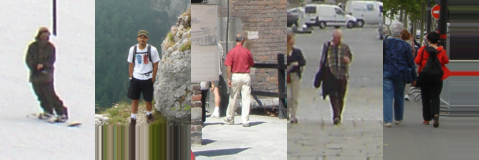
\includegraphics[width=0.8\textwidth]{ch3_inria.png}
\caption{Przykłady pozytywnych próbek ze zbioru INRIA}
\label{fig:inria}
\end{figure}

Ponadto, wszystkie obrazy będące częścią pozytywnego zbioru próbek, zawierają dodatkowy opis lokalizacji osób na nim w formacie \textit{Pascal Challenge} \cite{Pascal_Challenge}. Pozwala to na sprawdzenie poprawności działania finalnej metody.
Autorzy zbioru nie zapewnili negatywnego zbioru danych, odpowiadającego pozytywnym próbkom o rozmiarze 64x128 pikseli, pozostawiając wybór okien tego rozmiaru z większych negatywnych obrazów autorom konkretnej implementacji. Propozycja wyboru takich negatywnych okien została zaprezentowana w rozdziale \ref{sec:podzial}.


\section{Klasyfikator - Support Vector Machine}
\label{sec:svm}

Zadanie budowy klasyfikatora polega na podziale zbioru danych na dwa zestawy: treningowy i testowy. Każda próbka w zbiorze treningowym dostaje etykietę – jest próbką pozytywną, reprezentującą zajście jakiegoś zjawiska, lub negatywną – wtedy reprezentuje brak jego zajścia. Dla każdej próbki z obu zestawów wyliczana jest wartość deskryptora cech, po czym wraz z odpowiednią etykietą, pozytywną lub negatywną, przekazywana jest ona do klasyfikatora w celu wytrenowania go. Po tym kroku, możliwe jest dokonywanie klasyfikacji, na bardzo podobnej zasadzie do fazy treningowej. Klasyfikator na podstawie przekazanego wektora cech przewiduje do której z dwóch klas obiektów należy próbka – pozytywnej czy negatywnej.

Support Vector Machine (SVM) jest bardzo często używaną i dającą dobre wyniki techniką, statystycznego uczenia maszynowego. Metoda zaproponowana przez dwójkę C. Cortesa i V. Vapnika w pracy \cite{Cortes95}, z matematycznego punktu widzenia jest problemem optymalizacyjnym postaci:\\

\begin{enumerate}[label=\arabic*)]
  \item \rule{0pt}{1pt}\vspace*{-12pt}
    \begin{equation*} 
     \min_{\bm{w},b,\xi} \frac{1}{2} \bm{w}^T\bm{w} + C\sum_{i=1}^{l} \xi_{i}
    \end{equation*}
    przy ograniczeniach:
  \item \rule{0pt}{1pt}\vspace*{-12pt}
  	\begin{equation*} 
     {l}y_{i}(\bm{w}^{T}\phi(\bm{x}_i)+b)\geq 1-\xi_{i}
    \end{equation*}
   \item \rule{0pt}{1pt}\vspace*{-12pt}
  	\begin{equation*} 
     \xi_{i} \geq 0
   	\end{equation*}
   	gdzie zbiór treningowy to zbiór par
  \item \rule{0pt}{1pt}\vspace*{-12pt}
  	\begin{equation*} 
     (\bm{x}_i, y_i), i \in \{1, ..., l\}
   	\end{equation*}
   	wektorem cech dla danej próbki jest
   	\item \rule{0pt}{1pt}\vspace*{-12pt}
  	\begin{equation*} 
     \bm{x}_i \in R^n
   	\end{equation*}
   	a identyfikatorem klasy i-tej próbki jest
   	\item \rule{0pt}{1pt}\vspace*{-12pt}
  	\begin{equation*} 
     y_i \in \{-1, 1\}
   	\end{equation*}
\end{enumerate}

Intuicyjna ilustracja metody, na przykładzie dwuwymiarowego wektora cech została zaprezentowana na rysunku \ref{fig:svm}.

Wektory cech odwzorowywane są na przestrzeń o większej liczbie wymiarów poprzez funkcję $\phi$. Zadaniem SVM jest znalezienie takiego podziału hiperpłaszczyzny, jak najbardziej odległej od granic umiejscowienia wektorów obu klas. Funkcja $K(\bm{x}_i, \bm{x}_j) = \xi(\bm{x}_i)^T\xi(\bm{x}_j)$ nazywana jest funkcją jądra SVM (\textit{kernel}).

Najczęściej używanymi funkcjami są:
\begin{enumerate}[label=\arabic*)]
  \item \rule{0pt}{1pt}\vspace*{-12pt}
  funkcja liniowa:
    \begin{equation*} 
     K(\bm{x}_i, \bm{x}_j) = \bm{x}_i^T\bm{x}_j
    \end{equation*}
  \item \rule{0pt}{1pt}\vspace*{-12pt}
  funkcja wielomianowa:
    \begin{equation*} 
     K(\bm{x}_i, \bm{x}_j) = (\gamma\bm{x}_i^T\bm{x}_j+r)^d,  \gamma > 0
    \end{equation*}
  \item \rule{0pt}{1pt}\vspace*{-12pt}
  funkcja RBF:
    \begin{equation*} 
    K(\bm{x}_i, \bm{x}_j) = e^{-\gamma\Vert\bm{x}_i-\bm{x}_j\Vert^2},  \gamma > 0
    \end{equation*}
  \item \rule{0pt}{1pt}\vspace*{-12pt}
  esica (\textit{sigmoid}):
    \begin{equation*} 
    K(\bm{x}_i, \bm{x}_j) = tanh(-\gamma\bm{x}_i^T\bm{x}_j+r)
    \end{equation*}
  	gdzie $\gamma, r, d$ są parametrami.
\end{enumerate}

\begin{figure}[htb]
\centering
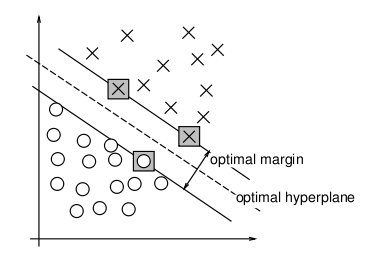
\includegraphics[width=0.5\textwidth]{ch3_svm.png}
\caption{Przykład budowy klasyfikatora dla wektora dwóch cech. \textit{Źródło: \cite{Cortes95}}}
\label{fig:svm}
\end{figure}

Zjawiskiem niepożądanym przy treningu klasyfikatora jest jego przetrenowanie. Do takiej sytuacji dochodzi w momencie, gdy w zbiorze treningowym którejś z klas znajduje się zbyt duża liczba wektorów leżących bardzo blisko realnej granicy. Wtedy hiperpłaszczyzna wyznaczona przez SVM jest dobrze dopasowana do tych skrajnych w przypadku jeden klasy i próbek drugiej klasy, leżących dalej od realnej granicy. W konsekwencji, wyznaczona granica może leżeć dość daleko od realnej.

\section{Podział zbioru danych}
\label{sec:podzial}

Jak wspomniano w \ref{sec:dane}, autorzy bazy danych INRIA zapewnili odpowiednio wykadrowany pozytywny zbiór treningowy i testowy, zawierający próbki o rozmiarze zgodnym z oknem detekcji, zawierające postać ludzką w samym jej centrum. Zbiory te zostały podzielone w stosunku 2416 próbek treningowych i 626 próbek testowych.
W przypadku zbiorów negatywnych, które zostały podzielone w stosunku 1218 próbek treningowych i 453 próbki testowe, mamy do czynienia z pełnymi zdjęciami w różnych rozdzielczościach. W tym przypadku, autorzy zbioru pozostawili dowolność w konstrukcji wykadrowanych zbiorów autorom konkretnej implementacji.

Proponowane podejście do generacji zarówno zbioru treningowego i testowego jest następujące.
Z~każdego obrazu ze zbioru negatywnego generowane są cztery okna o rozmiarze 64x128 pikseli - trzy całkowicie losowe i jedno wybierane według następującej zasady:
na całym obrazie stosowany jest operator Sobela w kierunkach poziomym i pionowym, wybierane jest to okno, dla którego suma wartości bezwzględnych takiej operacji jest maksymalna. Innymi słowy, wybierane jest okno, które na całym obrazie dominuje pod względem ilości krawędzi.

\begin{figure}[htb]
\centering
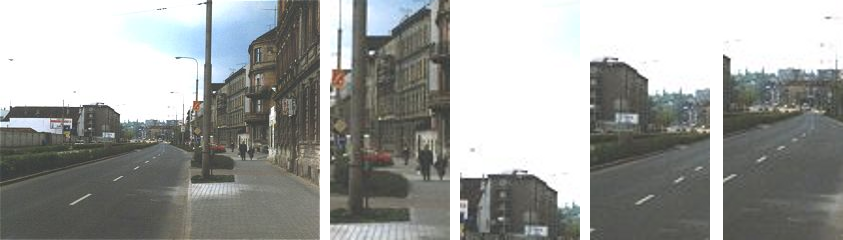
\includegraphics[width=0.8\textwidth]{ch3_sobel.png}
\caption{Negatywny obraz ze zbioru danych i wygenerowane na jego podstawie negatywne dane treningowe, od lewej: na podstawie wyniku filtru Sobela i 3 losowe okna}
\label{fig:sobel}
\end{figure}

Takie podejście powinno pozwolić na generację wiarygodnego klasyfikatora. Użyte negatywne dane, zarówno te wybrane do treningu klasyfikatora jak i jego walidacji, będą zróżnicowane pod względem ilości krawędzi, czyli cechy głównie wykorzystywanej przez prezentowane deskryptory do opisu obiektów.

Przykład negatywnego obrazu ze zbioru wraz z wygenerowanymi na jego podstawie oknami został przedstawiony na rys. \ref{fig:sobel}.

\section{Trening i walidacja}
\label{sec:trening}

Wytrenowanie klasyfikatora Support Vector Machine polega na konstrukcji wektora próbek - w kontekście tej pracy jest to wynik obliczenia danego deskryptora cech lub wynik połączenia kilku deskryptorów. Jeżeli wyjściem z deskryptora jest macierz, dokonuje się ''rozwinięcia'' tej macierzy w wektor poprzez połączenie ze sobą kolejnych wierszy lub kolumn. Przyjęty sposób zmiany rozmiaru macierzy nie ma znaczenia, gdyż każdy element wektora reprezentuje niezależną od innych cechę, ważne jest natomiast by zachować konsekwencję zarówno w trakcie budowy takiego wektora w fazie treningu jak i w fazie klasyfikacji. Każdemu wektorowi próbki przypisana jest etykieta oznaczająca klasę, do jakiej on należy. W pracy przyjęto następujący sposób etykietowania: do klasy \textit{0} należą wszystkie wektory, które są efektem zastosowania deskryptora na próbce nie zawierającej sylwetki ludzkiej, z kolei do klasy \textit{1} na próbce z sylwetką ludzką.

W pracy do budowy klasyfikatora użyto implementacji Support Vector Machine udostępnionej w~bibliotece OpenCV2. W trakcie badań uwzględniono budowę klasyfikatora z użyciem liniowego odwzorowania (tzw. \textit{kernel}) wektora próbki.

Klasyfikator nie posiada, w przeciwieństwie do danych ze zbioru treningowego, żadnych informacji na temat klasy, do jakiej należą poddawane przez nas klasyfikacji próbki ze zbioru testowego, dlatego też pierwszym sprawdzeniem poprawności działania klasyfikatora powinno być zastosowanie go na przygotowanym wcześniej zbiorze testowym. Znajomość procentowej poprawności odpowiedzi klasyfikatora pozwala krytycznie spojrzeć na poprawność zastosowanej metody i zauważyć pewne problemy jak np. przetrenowanie klasyfikatora, zanim dokona się sprawdzenia działania metody na rzeczywistych, bardziej złożonych danych.

W przypadku detekcji obiektów, takich jak ludzie, na obrazie, za zadowalający można przyjąć klasyfikator zapewniający ok. 90\% poprawności klasyfikacji zarówno na pozytywnym jak i negatywnym zbiorze testowym.

W przypadku Support Vector Machine, walidacja jest szczególnie ważna w przypadkach, w których używa się funkcji odwzorowującej wektor na wyższy wymiar. Wynika to z faktu, że dobór parametrów funkcji mapującej dokonywany jest na podstawie wyniku skuteczności klasyfikatora na zbiorze testowym.

\section{Dotrenowanie klasyfikatora}
\label{sec:dotrenowanie}

Skorzystanie z samego, wcześniej przygotowanego zbioru treningowego, może nie dawać zadowalających rezultatów w przypadku dokonywania klasyfikacji na rzeczywistych obrazach. Najczęstszą tego przyczyną jest fałszywa pozytywna detekcja w oknach, w których obserwowalne są kształty w pewnym sensie zbliżone do ludzkich, np. zawierające długie pionowe równoległe linie.
Przykłady kilku takich detekcji przedstawiono na rysunku \ref{fig:fp}.

W celu poprawienia skuteczności działania klasyfikatora dokonuje się jego dotrenowania. Polega ono na wykryciu fałszywych pozytywnych wskazań na testowym zbiorze obrazów rzeczywistych, a~następnie ponownym wytrenowaniu klasyfikatora, tym razem jednak ze zbiorem negatywnych próbek powiększonym o właśnie te niepoprawne detekcje.

\begin{figure}[htb]
\centering
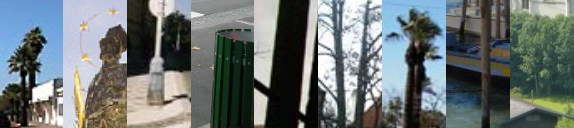
\includegraphics[width=0.8\textwidth]{ch3_fp.png}
\caption{Przykłady fałszywie pozytywnych detekcji}
\label{fig:fp}
\end{figure}

Negatywny zbiór treningowy jest jednak powiększany nie przez całość, a tylko część fałszywych pozytywnych okien wygenerowanych w fazie testu. Badania pokazały, że zbyt duży udział takich próbek w~całym negatywnym zbiorze treningowym prowadzi do zjawiska przetrenowania klasyfikatora, opisanego w \ref{sec:svm}. W związku z tym pierwotny zbiór treningowy powiększany jest np. o 1/3 losowych, wygenerowanych detekcji tego typu, po czym następuje ponowny trening klasyfikatora.


\section{Detekcja w przesuwnym oknie}
\label{sec:okno}

Ze względu na fakt, że rzeczywiste obrazy, na których dokonuje się detekcji obiektów, mogą mieć różne rozdzielczości, krokiem wymaganym na samym początku procesu detekcji, po wczytaniu obrazu powinna być pewna jego normalizacja. W niniejszej pracy, wszystkie obrazy wejściowe zmniejszane są do wysokości 600 pikseli, z zachowaniem proporcji. Dopiero na takim obrazie rozpoczynana jest detekcja obiektów.

Biorąc pod uwagę wymagania klasyfikatora, polegające na tym że klasyfikacji można poddać tylko i~wyłącznie okno o takim samym rozmiarze jak próbki poddane treningowi, niemożliwa jest klasyfikacja całego obrazu wejściowego w jednym kroku. Aby dokonać detekcji stosuje się koncepcję tzw. przesuwnego okna. Polega ona na podziale obrazu wejściowego na fragmenty o rozmiarze zgodnym z wielkością okna klasyfikowanego. Dla każdego takiego fragmentu dokonuje się osobnej, niezależnej od innych fragmentów, klasyfikacji. Takie niezłożone podejście ma jednak swoją wadę - ze względu na dużą liczbę testowanych okien w obrębie jednego obrazu, nawet wysoka celność klasyfikatora w przypadku próbek negatywnych może prowadzić do dużej liczby fałszywie pozytywnych detekcji (FP - \textit{False Positives}). Jest to zjawisko polegające na zaklasyfikowaniu próbki jako prawdziwej, podczas gdy w rzeczywistości jest ona fałszywa.

W badaniach przeprowadzonych w niniejszej pracy dokonano detekcji w oknie o rozmiarze 64x128 pikseli. Okno było przesuwane co 32 piksele w poziomie i co 64 piksele w pionie.

\section{Skalowanie obrazu testowanego}
\label{sec:skalowanie}

Biorąc pod uwagę to, że rzeczywiste obrazy testowane są zwykłymi fotografiami, zrobionymi w różnych okolicznościach, sylwetki ludzkie na nich obecne nie podlegają żadnej normalizacji.
Oznacza to, że człowiek, który powinien zostać wykryty na obrazie, może zajmować różną jego część, w zależności od tego jak daleko od miejsca zrobienia zdjęcia znajdował się w danej chwili. W testowym zbiorze danych obecne są przykłady zdjęć, w których postać znajduje się na pierwszym planie i jest obecna na prawie całej wysokości obrazu. Znajduje się w nim również wiele obrazów, w których postaci znajdują się w tle i wypełniają stosunkowo małą powierzchnię obrazu.

Przy stałej wielkości okna detekcji, która określona jest przez sposób budowy deskryptora cech w~trakcie treningu klasyfikatora, w celu wykrycia obiektów o różnej wielkości na obrazie, konieczne jest zatem kilkukrotne przeskalowanie obrazu testowanego.

\begin{figure}[htb]
\centering
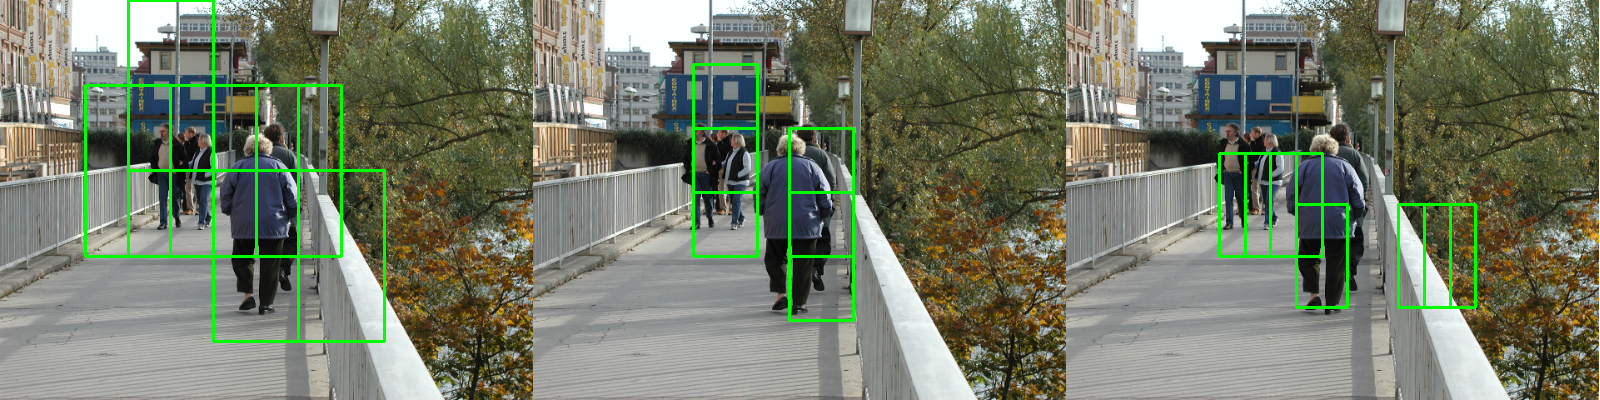
\includegraphics[width=0.8\textwidth]{ch3_scales.png}
\caption{Przykłady detekcji na obrazie testowanych w~skalach kolejno: \textbf{0.75}, \textbf{1} i \textbf{1.25}}
\label{fig:skale}
\end{figure}

Testy wykonane na obrazach przeskalowanych w skalach 0.25, 0.5, 0.75, 1 i 1.25 wykazały, że ostatecznie wystarczające będzie przeskalowanie obrazów testowanych w skalach \textbf{0.5}, \textbf{0.75} i \textbf{1}. W przypadku skali 0.25, pożądany obiekt był wykrywany w bardzo niewielkiej ilości przypadków, z kolei dla skali 1.25, ekstrakcja okien detekcji z dużym zbliżeniem, powodowała klasyfikację próbek z wieloma szczegółami obecnymi w otoczeniu. Konsekwencją tego była generacja znacznej liczby FP.

Na rysunku \ref{fig:skale} znajdują się przykłady detekcji obiektów na przeskalowanych obrazach testowych w skalach 0.75, 1 i 1.25.

\section{Eliminacja redundantnych detekcji}
\label{sec:eliminacja}

Detekcja obiektu na kilku przeskalowanych obrazach, a także mały krok przesunięcia przesuwnego okna może prowadzić do sytuacji, w której ten sam obiekt zostanie wykryty kilkukrotnie.
Aby w ostatecznym wyniku detekcji uniknąć tego typu sytuacji przyjęto następujący algorytm postępowania:
\\

\begin{algorithm}[H]
 \SetAlgoLined
 \KwData{zbiór okien detekcji zaklasyfikowanych pozytywnie przez klasyfikator w postaci \{współrzędne okna, pewność detekcji\}}
 \KwResult{zbiór ostatecznych okien detekcji}
 strefa zabroniona := $\oslash$\;
 finalny zbiór okien detekcji := $\oslash$\;
 posortuj wejściowe okna detekcji malejąco względem pewności detekcji\;
 
 \ForEach{okno}{
 	\If{okno = \{współrzędne, pewność\} $\notin$ strefa zabroniona}{
 	finalny zbiór okien detekcji := finalny zbiór okien detekcji $\cup$ okno\;
 	strefa zabroniona := strefa zabroniona $\cup$ współrzędne\;
 	}
 }
 \Return{finalny zbiór okien detekcji}
 \\
 \caption{Algorytm usuwania redundantnych detekcji}
\end{algorithm}

\begin{figure}[htb]
\centering
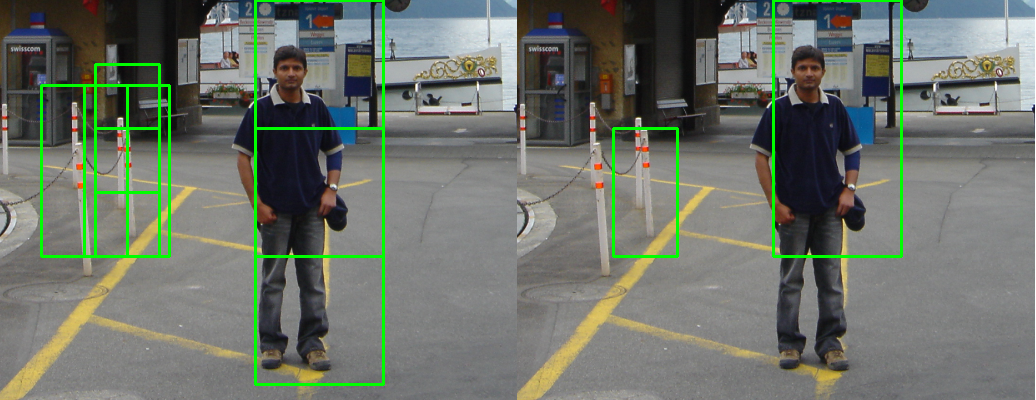
\includegraphics[width=0.8\textwidth]{ch3_redundant.png}
\caption{Po lewej obraz z redundantnymi detekcjami, po prawej po usunięciu redundantnych detekcji}
\label{fig:redundancje}
\end{figure}

Przykład pierwotnych, redundantnych okien detekcji wraz z oknami po redukcji, znajduje się na rysunku \ref{fig:redundancje}.

\section{Walidacja z wykorzystaniem danych rzeczywistych}
\label{sec:rzeczywiste}

Dzięki udostępnieniu, wraz z pozytywnymi zestawami (zawierającymi
przynajmniej jedną sylwetkę ludzką), zarówno zdjęć testowych jak i
treningowych w bazie INRIA plików opisu umiejscowienia tychże na
obrazie w formacie \textit{Pascal Challenge}, możliwe było zbudowanie
automatycznego narzędzia pozwalającego na przebadanie skuteczności
działania metody na obrazach jakie w rzeczywistości zostaną poddane
procesowi detekcji.

Przykładowy obraz z pozytywnego zbioru testowego z zaznaczonymi występującymi na nim sylwetkami ludzkimi znajduje się na rysunku \ref{fig:pascal}, z kolei odpowiadający mu plik
opisującym na nim obecność sylwetek ludzkich w formacie \textit{Pascal
Challenge} znajduje się poniżej (oryginalny obraz ma rozmiar 953 x 828
pikseli).

\begin{figure}[htb]
\centering
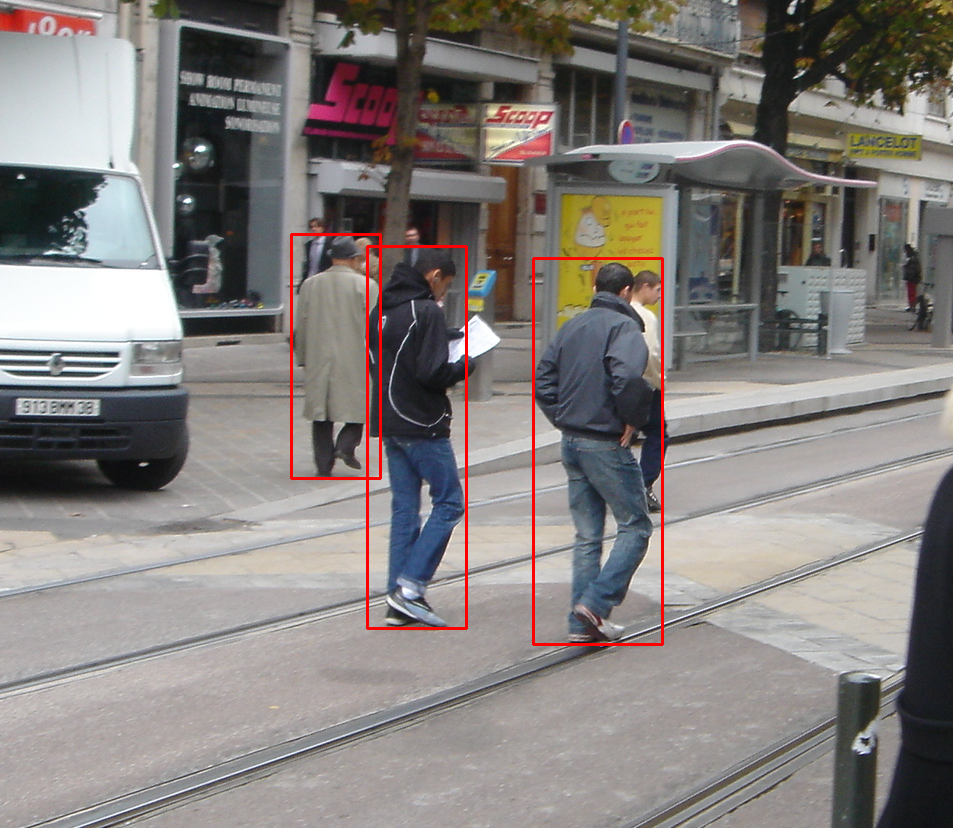
\includegraphics[width=0.8\textwidth]{ch4_pascal.png}
\caption{Przykładowy obraz z pozytywnego zbioru testowego z zaznaczonymi występującymi na nim postaciami na podstawie informacji zawartych w odpowiadającym mu pliku w formacie \textit{Pascal Challenge}}
\label{fig:pascal}
\end{figure}

\begin{lstlisting}
# PASCAL Annotation Version 1.00

Image filename : "Test/pos/crop001514.png"
Image size (X x Y x C) : 953 x 828 x 3
Database : "The INRIA Rhone-Alpes Annotated Person Database"
Objects with ground truth : 3 { "PASperson" "PASperson" "PASperson" }

# Note that there might be other objects in the image
# for which ground truth data has not been provided.

# Top left pixel co-ordinates : (0, 0)

# Details for object 1 ("PASperson")
# Center point -- not available in other PASCAL databases -- refers
# to person head center
Original label for object 1 "PASperson" : "UprightPerson"
Center point on object 1 "PASperson" (X, Y) : (436, 280)
Bounding box for object 1 "PASperson" (Xmin, Ymin) - (Xmax, Ymax) : (367, 246) - (467, 629)

# Details for object 2 ("PASperson")
# Center point -- not available in other PASCAL databases -- refers
# to person head center
Original label for object 2 "PASperson" : "UprightPerson"
Center point on object 2 "PASperson" (X, Y) : (345, 263)
Bounding box for object 2 "PASperson" (Xmin, Ymin) - (Xmax, Ymax) : (291, 234) - (381, 479)

# Details for object 3 ("PASperson")
# Center point -- not available in other PASCAL databases -- refers
# to person head center
Original label for object 3 "PASperson" : "UprightPerson"
Center point on object 3 "PASperson" (X, Y) : (609, 293)
Bounding box for object 3 "PASperson" (Xmin, Ymin) - (Xmax, Ymax) : (533, 258) - (663, 645)
\end{lstlisting}

Jak wspomniano w rozdziale \ref{sec:okno}, często w systemach
wizyjnych, których zadaniem jest wykrycie obiektów na obrazie, do detekcji stosowana jest koncepcja okna przesuwanego wzdłuż i wszerz testowanego obrazu. Klasyfikator klasyfikuje każde z nich
jako pozytywne lub negatywne. W celu stwierdzenia, czy rezultat, jaki uzyskano dla
okna w wyniku klasyfikacji jest poprawny w~kontekście
informacji zawartych w pliku zawierającym informacje o sylwetkach
obecnych na obrazie, przyjęto następującą procedurę postępowania:

\begin{algorithm}[H]
 \SetAlgoLined
 \KwData{współrzędne okna detekcji, współrzędne prostokątów opisujących obiekty obecne na obrazie}
 \KwResult{wartość logiczna odpowiadająca na pytanie, czy klasyfikacja jest poprawna czy też nie}
 \ForEach{prostokąt opisujący obiekt} {
 	\If{okno ma przynajmniej jeden punkt wspólny z prostokątem} {
 		\If{$pole(okno \cap prostokat) \geq \frac{1}{2} min(pole(okno), pole(prostokat))$} {
 			\Return{true}\;
 		}
 	}
 }
 \Return{false}
 \\
 \caption{Algorytm sprawdzenia czy okno poddane detekcji jest w rzeczywistości pozytywne czy negatywne}
\end{algorithm}

Na rysunku \ref{fig:detections} zaprezentowano przykład działania powyższego algorytmu, dokonując detekcji wykonywanych na kilkukrotnie przeskalowanym obrazie, bez uwzględnienia algorytmu redukcji. Kolorem czerwonym zaznaczony jest prostokąt opisujący obiekt na obrazie, na podstawie załączonego pliku. Kolorem niebieskim oznaczone są okna zaklasyfikowane jako fałszywie pozytywne detekcje. Kolorem zielonym oznaczone są okna zaklasyfikowane jako prawdziwie pozytywne detekcje.

\begin{figure}[htb]
\centering
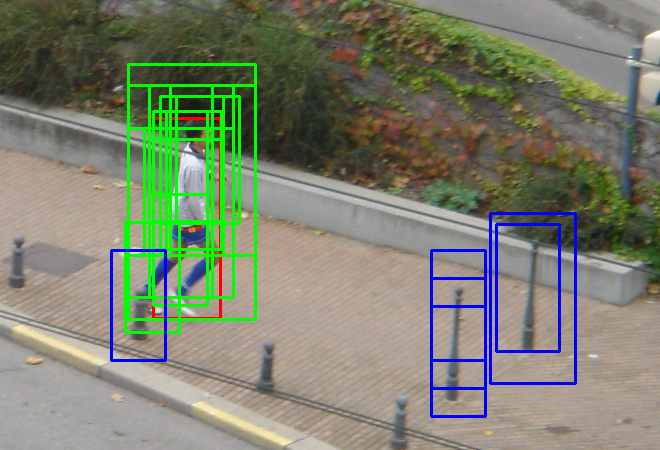
\includegraphics[width=0.9\textwidth]{ch4_dets.png}
\caption{Przykłady wyników klasyfikacji okien.}
\label{fig:detections}
\end{figure}


\section{Sposób bezpośredniego porównania metod}
\label{sec:porownanie}

Porównania skuteczności metod detekcji obiektów można dokonać poprzez
sprawdzenie jej działania na bardzo zróżnicowanym zbiorze testowym. W
kontekście tej pracy jest to zbiór różnych zdjęć, na których obecni są
ludzie w różnych pozach, w różnych częściach kadru, a także na
bardzo zróżnicowanym tle. Zastosowanie detekcji przy użyciu każdej z
poszczególnych metod pozwala na znalezienie zależności pomiędzy
odsetkiem fałszywych pozytywnych detekcji a skutecznością detekcji.
Sprawdzenie metody pod takim kątem pozwala na znalezienie konsensusu
pomiędzy stopniem fałszywych pozytywnych detekcji jakie można zaakceptować w konkretnym zastosowaniu, a celnością detekcji, jaką jesteśmy w stanie osiągnąć przy poszukiwaniu na obrazie konkretnej klasy obiektów. W rzeczywistych przypadkach bowiem,
z reguły nie ma się do czynienia ze wspomnianym przypadkiem detekcji na bardzo
zróżnicowanym zbiorze, lecz w stosunkowo niezmiennym środowisku, które
znane jest z góry. Wyznaczenie zależności pomiędzy częstością
występowania fałszywych pozytywnych detekcji w przypadku konkretnego
obrazu, a skutecznością metody pozwala zatem odpowiedź na pytanie - do
jakiego poziomu należałoby wytrenować klasyfikator, aby można było
uzyskać zadowalający oczekiwany stopień detekcji danej klasy obiektów.
Bardzo pomocnym narzędziem w tego typu analizie jest wyznaczenie
rozkładu błędu detekcji (DET - Detection error tradeoff), zaproponowanego w \cite{Martin97thedet}. Wykres, który służy do porównania między sobą klasyfikatorów binarnych, przedstawia zależność między odsetkiem fałszywych pozytywnych detekcji (reprezentowanej na osi odciętych wykresu), a stopniem nietrafionych pozytywnych detekcji danej metody (reprezentowanej na osi rzędnych wykresu). W przypadku dokonywania detekcji w przesuwnym oknie, jako odsetek fałszywych pozytywnych detekcji przyjmuje się rząd stosunku fałszywie pozytywnie zaklasyfikowanych okien do wszystkich badanych negatywnych okien (FPPW - False Positives Per Window). Wyższość jednej metody nad drugą, na podstawie wykresu DET, stwierdza się wtedy, gdy dla tych samych wartości fałszywie pozytywnych wskazań, wykres dla metody przyjmuje mniejszą wartość nietrafionych detekcji (krzywa opisująca rozkład lepszej metody jest na wykresie "pod" wykresem metody uznawanej za gorszą).

Oprócz tego, metody można bezpośrednio porównać wtedy i tylko wtedy
jeżeli dokona się detekcji w przesuwnym oknie z takim samym
przesunięciem okna w pionie i w poziomie w kolejnych detekcjach.
Ponieważ pożądana jest bardzo dokładne przebadanie zależności pomiędzy liczbą
FP a skutecznością detekcji liczba okien, w jakich
dokonywana jest detekcja przy użyciu każdej z metod powinna być taka
sama i możliwie jak największa.


\section{Analiza złożoności metod}
\label{sec:zlozonosc}

Zaproponowane metody różnią się między sobą m.in. operacjami matematycznymi potrzebnymi do obliczenia danego deskryptora czy długością wektora wynikowego.
Dlatego też, poza przeprowadzoną analizą jakościową,
przeprowadzono analizę czasową badanych metod. Badając każdą z nich
zmierzono czas, jaki był potrzebny dla wszystkich ww. etapów przeprowadzonych badań. Aby zapewnić wiarygodną porównywalność uzyskanych wyników wszystkie badania przeprowadzono na identycznej konfiguracji sprzętowej, a proces zajmujący się obliczeniami opisanymi w tym rozdziale był jedynym aktywnie działającym w systemie, przez co nie był on wywłaszczany przez inne procesy w kontekście czasu zajętości procesora.\\
Konfiguracja testowa była następująca:

\begin{itemize}
\item CPU: Intel(R) Xeon(R) CPU E5645 (4 x 2.40 GHz)
\item RAM: 14 GB
\item System operacyjny: Amazon Linux AMI 2012.09
\end{itemize}

W tym miejscu należy dodać, że sposób implementacji metod nie zapewniał zrównoleglenia ich obliczeń na wielu rdzeniach procesora. Toteż w trakcie uruchomienia testu, przy powyższej konfiguracji, w jednym czasie, aktywnie był wykorzystywany tylko i wyłącznie jeden rdzeń procesora.

\section{Podsumowanie}
\label{sec:podsmetodologia}
W celu podsumowania obranej metodologii przeprowadzonych badań, w tabeli \ref{tab:metodologia} zestawiono procedurę "krok po kroku" przyjętą w
metodologii analizy wybranych deskryptorów używanych w algorytmach
detekcji obiektów. Oprócz nazwanych etapów prowadzących do uzyskania
oceny danej metody uwzględniono informacje wejściowe potrzebne do
przeprowadzenia każdego z kolejnych kroków, jak i~informacje dostępne
na wyjściu, będące efektem przeprowadzenia danego etapu.

\begin{center}
    \begin{longtable}{ | l | p{4cm} | p{5cm} | p{5cm} |}
    \caption{Podsumowanie metodologii przyjętej w trakcie badania wybranych metod}
    \label{tab:metodologia}\\
    \hline
    Lp. & Nazwa kroku & Wejście & Wyjście \\ \hline
    1. & Generacja negatywnego zbioru testowego & Zbiór
negatywnych 1221 zdjęć (niezawierających sylwetek ludzkich) & Negatywne kadry treningowe 64x128 pikseli - kadr o największej ilości krawędzi
dla danego zdjęcia oraz 5 losowych kadrów \\ \hline

	2. & Ekstrakcja cech z pozytywnego zbioru treningowego &
	Pozytywny zbiór
kadrów treningowych o rozmiarze 64x128 pikseli 2419 &
	 Macierz
zawierająca 2419 wierszy, w każdym zawierająca wektor deskryptora cech \\ \hline

3. & Ekstrakcja cech z negatywnego zbioru treningowego &
   Negatywny zbiór
kadrów treningowych (wyjście z 1) o rozmiarze 64x128 pikseli &
Macierz
zawierająca 1221 wierszy, w każdym zawierająca wektor deskryptora cech \\ \hline

4. & Pierwszy trening klasyfikatora SVM &
Macierz cech pozytywnych (wyjście z 2) jako dane klasy 1, macierz cech
negatywnych (wyjście z 3) jako dane klasy 0 & Struktura SVM \\ \hline

5. & Walidacja krzyżowa pierwszego klasyfikatora & Struktura
wytrenowanego klasyfikatora SVM (wyjście z 4), zbiór pozytywnych (629) i
negatywnych (909)  kadrów testowych o rozmiarze 64x128 &
Skuteczność działania metody na pozytywnym i negatywnym zbiorze
testowym \\ \hline

6. & Znalezienie fałszywych pozytywnych wskazań dla metody & Zbiór
negatywnych (456) zdjęć & Negatywne kadry treningowe 64x128,
które pierwszy klasyfikator zaklasyfikował jako próbkę pozytywną\\ \hline

7. & Ekstrakcja cech ze zbioru fałszywych pozytywnych wskazań & Kadry
fałszywych pozytywnych wskazań dla metody & Macierz zawierająca n
wierszy, w każdym zawierająca wektor deskryptora cech\\ \hline

8. & Połączenie deskryptorów negatywnych cech & Macierz deskryptora
negatywnego zbioru treningowego (wyjście z 3, zawierająca 1221 wierszy),
macierz deskryptora fałszywych pozytywnych wskazań (wyjście z 7,
zawierająca m wierszy) & Wspólna macierz zawierająca 1221+m wierszy, w
każdym zawierająca wektor deskryptora cech \\ \hline

9. & Trening klasyfikatora SVM &
Macierz cech pozytywnych (wyjście z 2) jako dane klasy 1,  macierz
cech negatywnych (wyjście z 8) jako dane treningowe klasy 0 &
Dotrenowana struktura SVM\\ \hline

10. & Walidacja krzyżowa dotrenowanego klasyfikatora & Struktura
dotrenowanego klasyfikatora SVM,  zbiór pozytywnych i negatywnych
(629 + 909) kadrów testowych o rozmiarze 64x128 & Skuteczność
działania metody na pozytywnym i negatywnym zbiorze testowym po
dotrenowaniu \\ \hline

11. & Detekcja sylwetek ludzkich na obrazach testowych & Zestaw (629) obrazów testowych z sylwetkami ludzkimi wraz z opisem ich
umiejscowienia & Rozkład DET (liczba fałszywych pozytywnych detekcji do
stopnia celności) dla metody, wyniki detekcji dla poszczególnych
obrazów testowych\\ \hline
    
    \hline
    \end{longtable}
\end{center}
\chapter{Wybrane deskryptory cech}
\label{cha:deskryptory}

\section{HOG - Histogram of Oriented Gradients}
\label{sec:hog}

\subsection{Algorytm obliczenia deskryptora}

Algorytm obliczenia deskryptora cech HOG ma następującą postać:

\begin{algorithm}[H]
 \SetAlgoLined
 \KwData{obraz $n x m$ w przestrzeni barw RGB;\\$k$ - rozmiar komórki;\\$w$ - szerokość histogramu (tutaj 9)}
 \KwResult{wektor deskryptora cech o długości $\lfloor\frac{m}{k}\rfloor x \lfloor\frac{n}{k}\rfloor x w$}
 zamień przestrzeń barw RGB na skalę szarości\;
 oblicz gradient w obu kierunkach na obrazie np. używając maski  $\left[\begin{array}{ccc}1 & 0 & -1\end{array}\right]$\;
 dla każdego piksela obrazu oblicz długość wektora gradientu ($\sqrt{I_x^2 + I_y^2}$) oraz jego kąt, tak aby leżał w przedziale $[0; \pi]$ (wykorzystując funkcję $atan2(I_y, I_x)$)\;
 podziel obraz na komórki $k x k$\;
 dla każdej komórki utwórz histogram o szerokości $w$, gdzie cechą jest kąt z przedziału $[0; \pi]$, a liczebnością suma długości gradientów\;
 \ForEach{piksel $\in$ obraz}{
	dokonaj interpolacji dwuliniowej współrzędnych piksela względem środków czterech najbliższych komórek\;
	w histogramach odpowiadającym powyższym komórkom zwiększ liczebność kątom, po przeprowadzaniu interpolacji liniowej kąta odpowiadającemu pikselowi\;
 }
 dokonaj normalizacji każdej próbki (w niniejszej pracy jest to norma L2)\;
 połącz kolejne wiersze macierzy próbek w wektor\;
 \Return{wektor cech}\;
 \caption{Algorytm obliczenia deskryptora cech HOG}
\end{algorithm}

\subsection{Wyniki pierwszej walidacji}

W tabeli \ref{tab:hog_first} zestawiono wyniki krzyżowej walidacji pierwszego klasyfikatora wytrenowanego 
próbkami, uzyskanymi metodą HOG, w zależności od rozmiaru komórki, w której wyliczany był histogram orientacji gradientów.

\begin{center}
    \begin{longtable}{ | p{5cm} | p{3cm} | p{3cm} | p{3cm} |}
    \caption{Wyniki pierwszej walidacji krzyżowej przy użyciu deskryptora HOG}
    \label{tab:hog_first} \\
    \hline
	Rozmiar komórki & 8x8 & 12x12 & 16x16 \\ \hline
	Funkcja jądra SVM & liniowa & liniowa & liniowa  \\ \hline
    Długość wektora cech & 7308 & 800 & 512 \\ \hline
    Liczba pozytywnych detekcji w pozytywnym zbiorze testowym & 575 & 474 & 462 \\ \hline
    Liczba negatywnych detekcji w pozytywnym zbiorze testowym & 57 & 152 & 164 \\ \hline
    Celność metody w pozytywnym zbiorze testowym & \textbf{91,85\%} & \textbf{75,72\%} & \textbf{73,81\%} \\ \hline
    Liczba pozytywnych detekcji w negatywnych zbiorze testowym & 31 & 172 & 57 \\ \hline
    Liczba negatywnych detekcji w negatywnym zbiorze testowym & 875 & 734 & 849 \\ \hline
    Celność metody w negatywnym zbiorze testowym & \textbf{96,58\%} & \textbf{81,02\%} & \textbf{93,71\%} \\ \hline
    \end{longtable}
\end{center}

\subsection{Przykłady fałszywych detekcji}

Przeważającą część fałszywie pozytywnych detekcji uzyskiwanych metodą HOG są okna, w których występują pary długich, równoległych linii, przypominające ludzką sylwetkę czy elementy które kształtem przypominają ludzką twarz. Jest to spodziewany efekt, biorąc pod uwagę to jak budowany jest deskryptor cech (opisywany jest kształt na podstawie krawędzi obrazu wejściowego).
Liczby wygenerowanych fałszywie pozytywnych okien, w zależności od rozmiaru komórki, przedstawione zostały w tabeli \ref{tab:fp_hog}.
Przykładowe fałszywie pozytywne detekcje dla metody HOG zostały przedstawione na rysunku \ref{fig:fp_hog}.

\begin{figure}[htb]
\centering
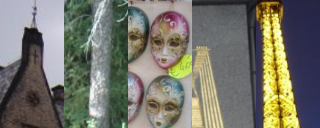
\includegraphics[width=0.8\textwidth]{hog_fps.png}
\caption{Przykłady fałszywie pozytywnych detekcji w metodzie HOG}
\label{fig:fp_hog}
\end{figure}

\begin{center}
    \begin{longtable}{ | p{5cm} | p{3cm} | p{3cm} | p{3cm} |}
    \caption{Liczba znalezionych fałszywie pozytywnych okien przy użyciu deskryptora HOG} \\
    \hline
	Rozmiar komórki & 8x8 & 12x12 & 16x16 \\ \hline
	Funkcja jądra SVM & liniowa & liniowa & liniowa  \\ \hline
    Liczba znalezionych pozytywnie fałszywych okien & 2759 & 14538 & 6446 \\ \hline
    \end{longtable}
    \label{tab:fp_hog}
\end{center}

\subsection{Wyniki drugiej walidacji}

W tabeli \ref{tab:hog_second} zestawiono wyniki krzyżowej walidacji klasyfikatora po dotrenowaniu pierwszego klasyfikatora fałszywie pozytywnymi detekcjami, wykrytymi w zbiorze testowym. W celu zminimalizowania efektu przetrenowania klasyfikatora wzięto pod uwagę tylko 25\% wygenerowanego zbioru.

\begin{center}
    \begin{longtable}{ | p{5cm} | p{3cm} | p{3cm} | p{3cm} |}
    \caption{Wyniki drugiej walidacji krzyżowej przy użyciu deskryptora HOG} 
    \label{tab:hog_second}\\
    \hline
	Rozmiar komórki & 8x8 & 12x12 & 16x16 \\ \hline
	Funkcja jądra SVM & liniowa & liniowa & liniowa  \\ \hline
    Liczba pozytywnych detekcji w pozytywnym zbiorze testowym & 531 & 445 & 223 \\ \hline
    Liczba negatywnych detekcji w pozytywnym zbiorze testowym & 95 & 181 & 403 \\ \hline
    Celność metody w pozytywnym zbiorze testowym & \textbf{84,82\%} & \textbf{71,09\%} & \textbf{35,62\%} \\ \hline
    Liczba pozytywnych detekcji w negatywnych zbiorze testowym & 32 & 79 & 290 \\ \hline
    Liczba negatywnych detekcji w negatywnym zbiorze testowym & 874 & 827 & 614 \\ \hline
    Celność metody w negatywnym zbiorze testowym & \textbf{96,47\%} & \textbf{91,28\%} & \textbf{67,77\%} \\ \hline
    \end{longtable}
\end{center}

\clearpage

\subsection{Rozkłady błędów detekcji}

Wykres rozkładu błędu detekcji dla metody HOG zaprezentowany został na rysunku \ref{fig:hog_det}.
Na osi odciętych wykresu znajduje się rząd stosunku fałszywych pozytywnych detekcji klasyfikatora i wszystkich negatywnych testowanych okien, na osi rzędnych zaś, średni odsetek błędu klasyfikatora w detekcji pozytywnego okna. Na podstawie wykresu można wyciągnąć wniosek, że w przypadku użycia liniowej funkcji jądra klasyfikatora SVM, najlepsze zachowanie prezentuje klasyfikator zbudowany przy deskryptora HOG wyliczanego na komórkach o rozmiarze 8x8 pikseli. Zachowuje on bardzo dobry wynik detekcji obiektu (ok. 95\%), w przypadku, gdy liczba FPPW jest rzędu $10^{-2}$. Na podstawie wykresu można również stwierdzić, że przy wyliczaniu bloków o rozmiarze 16x16 pikseli deskryptor HOG jest złym deskryptorem, a stopień jego błędu detekcji rośnie aż do 70\% przy FPPW rzędu $10^{-3}$.

\begin{figure}[htb]
\centering
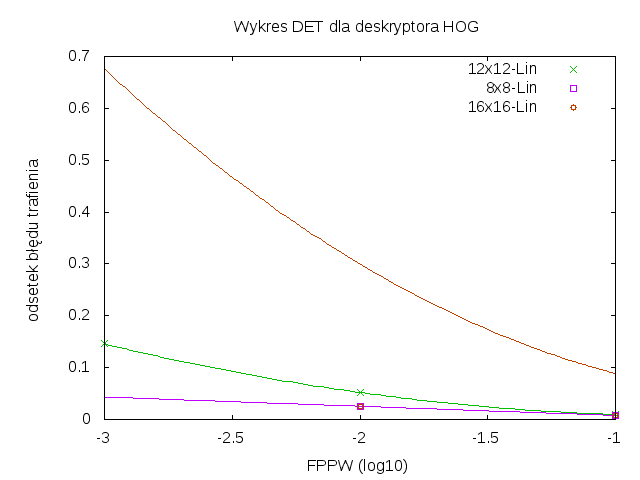
\includegraphics[width=0.9\textwidth]{hog_det.png}
\caption{Rozkład błędu detekcji dla różnych przyjętych komórek}
\label{fig:hog_det}
\end{figure}

\subsection{Analiza złożoności poszczególnych kroków metody}

W tabeli \ref{tab:hog_times} zestawiono czasy wykonywania poszczególnych kroków metodologii, w zależności od rozmiaru komórki deskryptora HOG, na konfiguracji testowej.

\begin{center}
    \begin{longtable}{ | p{5cm} | p{3cm} | p{3cm} | p{3cm} |}
    \caption{Czas wykonywania poszczególnych etapów badania metody HOG}
    \label{tab:hog_times}\\
    \hline
	Rozmiar komórki & 8x8 & 12x12 & 16x16 \\ \hline
	Funkcja jądra SVM & liniowa & liniowa & liniowa  \\ \hline
    Ekstrakcja cech pozytywnych / próbka & 6,23 ms & 5,67 ms & 5,19 ms \\ \hline
    Ekstrakcja cech negatywnych / próbka & 5,27 ms & 4,80 ms & 4,28 ms \\ \hline
    Pierwszy trening klasyfikatora & 33,69 s & 12,67 s & 8,14 s \\ \hline
    Generacja fałszywie pozytywnych okien & 590,40 s & 455,72 s & 409,20 s \\ \hline
    Drugi trening klasyfikatora & 40,62 s & 18,88 s & 10,36 s \\ \hline
    Analiza rozkładu błędu detekcji w zbiorze testowym & 1938 s & 1353 s & 1228 s \\ \hline
    \end{longtable}
\end{center}

\subsection{Podsumowanie}

Na podstawie uzyskanych wyników można stwierdzić, że najskuteczniejszą z przetestowanych wielkości komórki w deskryptorze HOG jest ta o rozmiarze 8x8 pikseli. Jako jedyna daje ona rozsądne wyniki przy obydwu walidacjach klasyfikatora. Również rozkład DET dla takiej wielkości komórki sugeruje wysoką skuteczność działania.

\clearpage

\section{Macierz kowariancji cech}
\label{sec:cov}

\subsection{Algorytm obliczenia deskryptora}

Algorytm obliczenia deskryptora cech, wykorzystującego macierz kowariancji ma następującą postać:

\begin{algorithm}[H]
 \SetAlgoLined
 \KwData{obraz $n x m$ w przestrzeni barw RGB;\\$k$ - rozmiar lokalnego bloku}
 \KwResult{wektor deskryptora cech o długości $\lfloor\frac{m}{k}\rfloor x \lfloor\frac{n}{k}\rfloor x 6^{2}$}
 macierz próbek := $\left[\begin{array}{ccc}\end{array}\right]$\;
 zamień przestrzeń barw RGB na skalę szarości\;
 podziel obraz na bloki $k x k$\;
 \ForEach{blok}{
	$I_x$ := jednokrotny operator Sobela dla bloku w kierunku poziomym\;
	$I_y$ := jednokrotny operator Sobela dla bloku w kierunku pionowym\;
	$I_{xx}$ := dwukrotny operator Sobela dla bloku w kierunku poziomym\;
	$I_{yy}$ := dwukrotny operator Sobela dla bloku w kierunku pionowym\;
	macierz cech := $\left[\begin{array}{ccc}\end{array}\right]$\;
	\ForEach{piksel $\in$ okno} {
		wektor cech := $\left[\begin{array}{cccccc}\vert I_x \vert & \vert I_y \vert & \vert I_{xx} \vert & \vert I_{yy} \vert & \sqrt{I_x^2 + I_y^2} & atan2(I_y, I_x)\end{array}\right]$\;
		dodaj wektor cech jako wiersz do macierzy cech\;
	}
	oblicz macierz kowariancji macierzy cech\;
	połącz kolejne wiersze macierzy cech w jeden wektor\;
	dodaj wektor do macierzy próbek\;
 }
 dokonaj normalizacji każdej próbki (w niniejszej pracy jest to norma L2)\;
 połącz kolejne wiersze macierzy próbek w wektor\;
 \Return{wektor cech}\;
 \caption{Algorytm obliczenia deskryptora cech, wykorzystującego macierz kowariancji}
\end{algorithm}

\subsection{Wyniki pierwszej walidacji}

W tabeli zestawiono wyniki krzyżowej walidacji pierwszego klasyfikatora wytrenowanego 
próbkami, uzyskanymi na podstawie wyliczenia deskryptora cech, wykorzystującego macierz kowariancji, w zależności od rozmiaru bloku na obrazie, w którym liczono macierz kowariancji.

\begin{center}
    \begin{longtable}{ | p{5cm} | p{3cm} | p{3cm} | p{3cm} |}
    \caption{Wyniki pierwszej walidacji krzyżowej przy użyciu deskryptora wykorzystującego macierz kowariancji cech}
    \label{tab:cov_first}\\
    \hline
	Rozmiar bloku & 8x8 & 16x16 & 24x24 \\ \hline
	Funkcja jądra SVM & liniowa & liniowa & liniowa  \\ \hline
    Długość wektora cech & 4608 & 832 & 360 \\ \hline
    Liczba pozytywnych detekcji w pozytywnym zbiorze testowym & 599 & 593 & 584 \\ \hline
    Liczba negatywnych detekcji w pozytywnym zbiorze testowym & 27 & 33 & 42 \\ \hline
    Celność metody w pozytywnym zbiorze testowym & \textbf{95,69\%} & \textbf{94,73\%} & \textbf{93,29\%} \\ \hline
    Liczba pozytywnych detekcji w negatywnych zbiorze testowym & 21 & 30 & 29 \\ \hline
    Liczba negatywnych detekcji w negatywnym zbiorze testowym & 885 & 876 & 877 \\ \hline
    Celność metody w negatywnym zbiorze testowym & \textbf{97,68\%} & \textbf{96,69\%} & \textbf{96,80\%} \\ \hline
    \end{longtable}
\end{center}

\subsection{Przykłady fałszywych detekcji}

Podobnie jak w przypadku metody HOG, zdecydowaną część zbioru fałszywie pozytywnych detekcji stanowiły okna, w których znajdowały się obiekty mające kształty przypominające ludzkie sylwetki, czyli np. obiekty zajmujące większość część okna, posiadające parę długich, równoległych krawędzi, jak słup czy drzewo.
Liczby wygenerowanych fałszywie pozytywnych okien, w zależności od rozmiaru komórki, przedstawione zostały w tabeli \ref{tab:fp_cov}.
Przykładowe fałszywie pozytywne detekcje dla metody opierającej się na liczeniu macierzy kowariancji cech, zostały przedstawione na rysunku \ref{fig:fp_cov}.

\begin{figure}[htb]
\centering
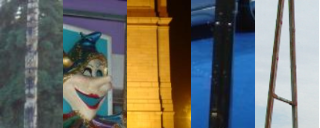
\includegraphics[width=0.8\textwidth]{cov_fps.png}
\caption{Przykłady fałszywie pozytywnych detekcji w metodzie korzystającej z macierzy kowariancji cech}
\label{fig:fp_cov}
\end{figure}

\begin{center}
    \begin{longtable}{ | p{5cm} | p{3cm} | p{3cm} | p{3cm} |}
    \caption{Liczba znalezionych fałszywie pozytywnych okien przy użyciu macierzy kowariancji cech} \\
    \hline
	Rozmiar komórki & 8x8 & 16x16 & 24x24 \\ \hline
	Funkcja jądra SVM & liniowa & liniowa & liniowa  \\ \hline
    Liczba znalezionych pozytywnie fałszywych okien & 4271 & 4141 & 7513 \\ \hline
    \end{longtable}
    \label{tab:fp_cov}
\end{center}

\subsection{Wyniki drugiej walidacji}

W \ref{tab:cov_second} tabeli zestawiono wyniki krzyżowej walidacji klasyfikatora po dotrenowaniu pierwszego klasyfikatora fałszywymi pozytywnymi detekcjami, wykrytymi w zbiorze testowym. W celu zminimalizowania efektu przetrenowania klasyfikatora wzięto pod uwagę 25\% fałszywie pozytywnych detekcji wygenerowanych na zbiorze testowym.

\begin{center}
    \begin{longtable}{ | p{5cm} | p{3cm} | p{3cm} | p{3cm} |}
    \caption{Wyniki drugiej walidacji krzyżowej przy użyciu deskryptora wykorzystującego macierz kowariancji cech}
    \label{tab:cov_second} \\
    \hline
	Rozmiar bloku & 8x8 & 16x16 & 24x24 \\ \hline
	Funkcja jądra SVM & liniowa & liniowa & liniowa  \\ \hline
    Liczba pozytywnych detekcji w pozytywnym zbiorze testowym & 571 & 502 & 289 \\ \hline
    Liczba negatywnych detekcji w pozytywnym zbiorze testowym & 55 & 124 & 337 \\ \hline
    Celność metody w pozytywnym zbiorze testowym & \textbf{91,21\%} & \textbf{80,20\%} & \textbf{46,17\%} \\ \hline
    Liczba pozytywnych detekcji w negatywnych zbiorze testowym & 14 & 19 & 15 \\ \hline
    Liczba negatywnych detekcji w negatywnym zbiorze testowym & 892 & 887 & 891 \\ \hline
    Celność metody w negatywnym zbiorze testowym & \textbf{98,45\%} & \textbf{97,90\%} & \textbf{98,34\%} \\ \hline
    \end{longtable}
\end{center}


\subsection{Rozkłady błędów detekcji}

Wykres rozkładu błędu detekcji zaprezentowany został na rysunku \ref{fig:cov_det}. Na podstawie wykresu można wyciągnąć wniosek, że w przypadku użycia liniowej funkcji jądra klasyfikatora SVM, najlepsze zachowanie prezentuje klasyfikator zbudowany przy użyciu macierzy kowariancji wyliczanej na blokach 16x16. Zachowuje on rozsądny wynik detekcji obiektu, gdy ma on do czynienia z obrazem, gdzie liczba FPPW jest rzędu $10^{-2}$, a wraz z malejącą liczbą fałszywych pozytywnych detekcji, odsetek błędu detekcji nie rośnie zbyt gwałtownie, jak np. w przypadku deskryptora zbudowanego o macierz kowariancji wyliczaną na blokach 8x8.

\begin{figure}[htb]
\centering
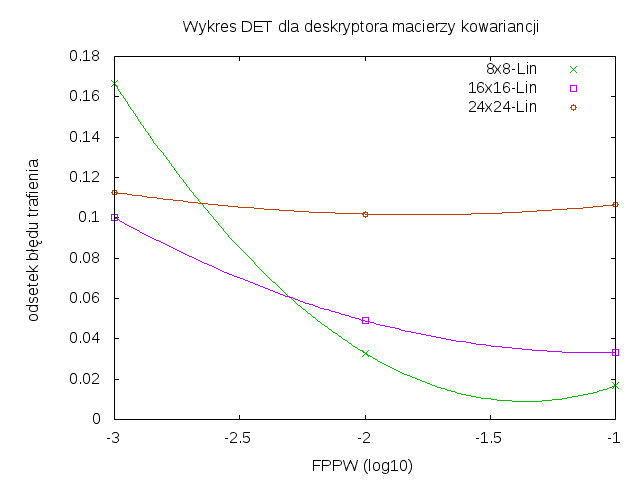
\includegraphics[width=0.9\textwidth]{cov_det.png}
\caption{Rozkład błędu detekcji dla różnych przyjętych wielkości macierzy}
\label{fig:cov_det}
\end{figure}

\subsection{Analiza złożoności poszczególnych kroków metody}

W tabeli \ref{tab:cov_times} zestawiono czasy wykonywania poszczególnych kroków metodologii, w zależności od rozmiaru bloku, z którego wyliczana jest macierz kowariancji, na konfiguracji testowej.

\begin{center}
    \begin{longtable}{ | p{5cm} | p{3cm} | p{3cm} | p{3cm} |}
    \caption{Czas wykonywania poszczególnych etapów badania metody opartej na macierzy kowariancji cech}
    \label{tab:cov_times}\\
    \hline
	Rozmiar bloku & 8x8 & 16x16 & 24x24 \\ \hline
	Funkcja jądra SVM & liniowa & liniowa & liniowa  \\ \hline
    Ekstrakcja cech pozytywnych / próbka & 11,12 ms & 4,33 ms & 3,51 ms \\ \hline
    Ekstrakcja cech negatywnych / próbka & 10,37 ms & 3,54 ms & 2,68 ms \\ \hline
    Pierwszy trening klasyfikatora & 50,81 s & 10,75 s & 5,99 s \\ \hline
    Generacja fałszywie pozytywnych okien & 909,12 s & 296,06 s & 231,88 s \\ \hline
    Drugi trening klasyfikatora & 68,49 s & 14,41 s & 8,79 s \\ \hline
    Analiza rozkładu błędu detekcji w zbiorze testowym & 3172 s & 912 s & 669 s \\ \hline
    \end{longtable}
\end{center}


\subsection{Podsumowanie}
Analizując powyższe wyniki można dojść do wniosku, że wielkościami bloków, dla których metoda daje rozsądne wyniki są bloki 8x8 pikseli i 16x16 pikseli. Użycie bloku 8x8 daje co prawda lepsze jakościowo wyniki w większości przypadków testowych, jednak jest to dużo bardziej kosztowne czasowo niż w przypadku bloku 16x16. Wynika to bezpośrednio z długości wektora cech, jaki powstaje w pierwszym przypadku. Deskryptor zbudowany na blokach o wielkości 24x24 pikseli jest złym deskryptorem i ma tendencję do szybkiego przetrenowania klasyfikatora.

\clearpage

\section{LBP - Local Binary Patterns}
\label{sec:lbp}

\subsection{Wprowadzenie}
W pracy \cite{Mu08} zaprezentowano metodę budowy deskryptora cech opartego na oryginalnym algorytmie Local Binary Patterns, dającego jednak lepsze wyniki w problemach detekcji kształtów, niż metoda, która pierwotnie opracowana została do detekcji tekstur. Wprawdzie pierwsze testy tej metody dawały obiecujące wyniki, jednak przy treningu klasyfikatora znacznie większymi zbiorami danych pokazały, że tak zbudowany deskryptor ma tendencję do przetrenowywania klasyfikatora.
W~związku z tym, w pracy zdecydowano się użyć tradycyjnej metody LBP.

\subsection{Algorytm obliczenia deskryptora}

Algorytm obliczenia deskryptora cech, wykorzystującego metodę LBP ma następującą postać:

\begin{algorithm}[H]
 \SetAlgoLined
 \KwData{obraz $n x m$ w przestrzeni barw RGB;\\$k$ - rozmiar lokalnego bloku;\\$p$ - próg tworzenia wzorca}
 \KwResult{wektor deskryptora cech o długości $\lfloor\frac{m}{k}\rfloor x \lfloor\frac{n}{k}\rfloor x 512$}
 macierz próbek := $\left[\begin{array}{ccc}\end{array}\right]$\;
 zamień przestrzeń barw RGB na skalę szarości\;
 podziel obraz na bloki $kxk$\;
 \ForEach{blok}{
 	w := zerowy wektor, 512-elementowy\;
	\ForEach{piksel $\in$ blok} {
		v := zerowy wektor, 8-elementowy\;
		\ForEach{sąsiad $\in$ wektor (po okręgu)} {
			\If{$\vert sasiad - piksel\vert > p$} {
				$v(sasiad) := 1$\;
			}	
		}
		n := liczba odpowiadająca binarnej reprezentacji w v\;
		$w(n) := w(n)+1$\;
	}
	dodaj wektor w do macierzy próbek\;
 }
 dokonaj normalizacji każdej próbki (w niniejszej pracy jest to norma L2)\;
 połącz kolejne wiersze macierzy próbek w wektor\;
 \Return{wektor cech}\;
 \caption{Algorytm obliczenia deskryptora cech w metodzie LBP}
\end{algorithm}

\subsection{Wyniki pierwszej walidacji}

W tabeli \ref{tab:lbp_first} zestawiono wyniki krzyżowej walidacji pierwszego klasyfikatora wytrenowanego 
próbkami, uzyskanymi na podstawie wyliczenia deskryptora cech metodą LBP, w zależności od rozmiaru bloku na obrazie, w którym liczono histogram rozkładu wzorca.

\begin{center}
    \begin{longtable}{ | p{5cm} | p{3cm} | p{3cm}|}
    \caption{Wyniki pierwszej walidacji krzyżowej przy użyciu deskryptora LBP}
    \label{tab:lbp_first}\\
    \hline
	Rozmiar bloku & 32x32 & 64x64 \\ \hline
	Funkcja jądra SVM & liniowa & liniowa \\ \hline
    Długość wektora cech & 4096 & 1024 \\ \hline
    Liczba pozytywnych detekcji w pozytywnym zbiorze testowym & 531 & 443 \\ \hline
    Liczba negatywnych detekcji w pozytywnym zbiorze testowym & 95 & 183 \\ \hline
    Celność metody w pozytywnym zbiorze testowym & \textbf{84,82\%} & \textbf{70,77\%}\\ \hline
    Liczba pozytywnych detekcji w negatywnych zbiorze testowym & 20 & 30 \\ \hline
    Liczba negatywnych detekcji w negatywnym zbiorze testowym & 886 & 876 \\ \hline
    Celność metody w negatywnym zbiorze testowym & \textbf{97,79\%} & \textbf{96,69\%} \\ \hline
    \end{longtable}
\end{center}

\subsection{Przykłady fałszywych detekcji}

Zbiór fałszywie pozytywnych detekcji uzyskanych w trakcie testowania metody LBP zawiera okna z~różnymi skomplikowanymi kształtami, zawierającymi dużą ilość różnie zorientowanych krawędzi. Przeważnie obiekty te kontrastują dość wyraźnie z tłem. Podobieństwo wykrytych pozytywnie negatywnych okien nie jest tak oczywiste jak w przypadku poprzednich dwóch metod, ma to jednak podstawy w~sposobie budowy deskryptora - opisuje on teksturę a nie kształt.
Liczby wygenerowanych fałszywie pozytywnych okien, w zależności od rozmiaru bloku, przedstawione zostały w tabeli \ref{tab:fp_lbp}.
Przykładowe fałszywie pozytywne detekcje dla metody LBP, zostały przedstawione na rysunku \ref{fig:fp_lbp}.

\begin{figure}[htb]
\centering
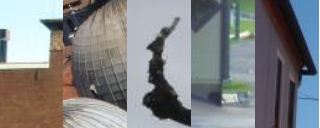
\includegraphics[width=0.8\textwidth]{lbp_fps.png}
\caption{Przykłady fałszywie pozytywnych detekcji w metodzie LBP}
\label{fig:fp_lbp}
\end{figure}

\begin{center}
    \begin{longtable}{ | p{5cm} | p{3cm} | p{3cm} |}
     \caption{Ilość znalezionych fałszywie pozytywnych okien przy użyciu deskryptora zbudowanego na podstawie macierzy kowariancji} \\
    \hline
	Rozmiar bloku & 32x32 & 64x64\\ \hline
	Funkcja jądra SVM & liniowa & liniowa   \\ \hline
    Ilość znalezionych pozytywnie fałszywych okien & 4711 & 5292 \\ \hline
    \end{longtable}
    \label{tab:fp_lbp}
\end{center}

\subsection{Wyniki drugiej walidacji}

W tabeli \ref{tab:lbp_second} zestawiono wyniki krzyżowej walidacji klasyfikatora po dotrenowaniu pierwszego klasyfikatora fałszywymi pozytywnymi detekcjami, wykrytymi w zbiorze testowym. W celu zminimalizowania efektu przetrenowania klasyfikatora wzięto pod uwagę 25\% fałszywie pozytywnych detekcji wygenerowanych na zbiorze testowym.

\begin{center}
    \begin{longtable}{ | p{5cm} | p{3cm} | p{3cm} |}
    \caption{Wyniki drugiej walidacji krzyżowej przy użyciu deskryptora LBP}
    \label{tab:lbp_second}\\
    \hline
	Rozmiar bloku & 32x32 & 64x64 \\ \hline
	Funkcja jądra SVM & liniowa & liniowa  \\ \hline
    Liczba pozytywnych detekcji w pozytywnym zbiorze testowym & 479 & 512 \\ \hline
    Liczba negatywnych detekcji w pozytywnym zbiorze testowym & 147 & 134 \\ \hline
    Celność metody w pozytywnym zbiorze testowym & \textbf{76,52\%} & \textbf{81,79\%} \\ \hline
    Liczba pozytywnych detekcji w negatywnych zbiorze testowym & 3 & 30 \\ \hline
    Liczba negatywnych detekcji w negatywnym zbiorze testowym & 903 & 876 \\ \hline
    Celność metody w negatywnym zbiorze testowym & \textbf{99,67\%} & \textbf{96,69\%} \\ \hline
    \end{longtable}
\end{center}


\subsection{Rozkłady błędów detekcji}

Wykres rozkładu błędu detekcji zaprezentowany został na rysunku \ref{fig:lbp_det}. Analizując wykres można dojść do wniosku, że oba przetestowane wielkości bloków, w których liczonych jest histogram metody LBP dają zbliżone do siebie rezultaty pod kątem celności detekcji.

\begin{figure}[htb]
\centering
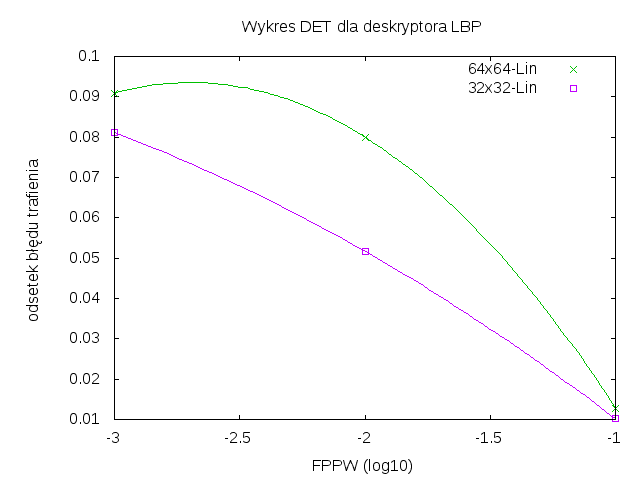
\includegraphics[width=0.9\textwidth]{lbp_det.png}
\caption{Rozkład błędu detekcji dla różnych przyjętych wielkości bloków}
\label{fig:lbp_det}
\end{figure}

\subsection{Analiza złożoności poszczególnych kroków metody}

W tabeli \ref{tab:lbp_times} zestawiono czasy wykonywania poszczególnych kroków metodologii, w zależności od rozmiaru bloku, w której wyliczany jest histogram metody LBP.

\begin{center}
    \begin{longtable}{ | p{5cm} | p{3cm} | p{3cm}|}
     \caption{Czas wykonywania poszczególnych etapów badania metody LBP} 
     \label{tab:lbp_times}\\
    \hline
	Rozmiar bloku & 32x32 & 64x64 \\ \hline
	Funkcja jądra SVM & liniowa & liniowa  \\ \hline
    Ekstrakcja cech pozytywnych / próbka & 14,10 ms & 11,08 ms \\ \hline
    Ekstrakcja cech negatywnych / próbka & 12,42 ms & 10,19 ms \\ \hline
    Pierwszy trening klasyfikatora & 79 s & 27,67 s \\ \hline
    Generacja fałszywie pozytywnych okien & 917,78 s & 657 s \\ \hline
    Drugi trening klasyfikatora & 89,83 s & 31,62 s \\ \hline
    Analiza rozkładu błędu detekcji w zbiorze testowym & 4831 s & 4914 s \\ \hline
    \end{longtable}
\end{center}


\subsection{Podsumowanie}
Podsumowując przeprowadzone testy, można zauważyć że pod względem jakościowym oba przetestowane rozmiary bloku, w którym na obrazie wyliczany jest histogram rozkładu wzorca, dają podobne rezultaty. W przypadku bloku 32x32 piksele jednak, poziom detekcji jest nieco wyższy w przypadku gdy rząd FPPW wynosi $10^{-2}$. Biorąc jednak pod uwagę rozmiar wektora cech, jaki powstaje przy ich ekstrakcji, słuszniejszym wyborem wydaje się być blok o rozmiarze 64x64, gdzie długość wektora cech jest 4 mniejsza od bloku 32x32. W konsekwencji, trening SVM zajmuje krótszy czas.

\clearpage

\section{Edgelets}
\label{sec:edge}

\subsection{Wprowadzenie}
Algorytm zaproponowany przez autorów metody, B. Wu i R. Nevatię w pracy \cite{Wu05} nie jest typowym deskryptorem cech opisującym obraz w postaci wektora. Zaproponowana metoda polega na budowie kaskadowego klasyfikatora, porównującego w każdym kroku podobieństwo fragmentu obrazu do każdego z wielu przygotowanych wcześniej wzorcowych kształtów. Ponieważ SVM, klasyfikator używany w tej pracy, jest mocnym klasyfikatorem, potrzebującym do treningu i klasyfikacji wektora zawierającego całość informacji, w niniejszej pracy dokonana została próba przystosowania metody do użycia właśnie z wykorzystaniem takiego rodzaju klasyfikatora.

Ze względu na bardzo wysoką złożoność metody, w przypadku porównywania z wieloma wzorcowymi kształtami, na podstawie zbioru treningowego, wygenerowano po 150 losowych masek dla fragmentów obrazu o rozmiarze 3x3, 4x4 i 5x5 i na ich podstawie dokonywano obliczenia deskryptora.


\subsection{Algorytm obliczenia deskryptora}

Proponowany algorytm obliczenia deskryptora cech, bazujący na oryginalnej metodzie \textit{Edgelets} ma następującą postać:

\begin{algorithm}[H]
 \SetAlgoLined
 \KwData{obraz $n x m$ w przestrzeni barw RGB;\\$k$ - rozmiar maski, względem której dokonywane jest porównywanie;\\macierz wzorcowych masek ($l x k^2$)}
 \KwResult{wektor deskryptora cech o długości $l$}
 zamień przestrzeń barw RGB na skalę szarości\;
 oblicz gradient w obu kierunkach na obrazie np. używając maski  $\left[\begin{array}{ccc}1 & 0 & -1\end{array}\right]$\;
 oblicz długość wektora gradientu w każdym pikselu\;
 dokonaj dyskretyzacji kąta gradientu w każdym pikselu: $round(\frac{atan2(I_y, I_x)*6}{\pi})$\;
 $L := [1, 0.8, 0.5, 0, 0.5, 0.8]$\;
 \ForEach{pikselobrazu $\in$ obraz, pikselobrazu $\in \{0,1,..,5\}$}{
	\ForEach{maska wzorcowa} {
	ocena := 0\;
		\ForEach{pikselmaski $\in$ maska, pikselmaski $\in \{0,1,..,5\}$}{
			ocena := ocena + $\sqrt{I_x^2+I_y^2} * L[\vert piksel obrazu - piksel maski\vert+1]$\; 
		}
	wektor(maska) := wektora(maska) + ocena\;
	}
 }
 \Return{wektor cech}\;
 \caption{Proponowany algorytm deskryptora cech, wykorzystujący metodę Edgelets}
\end{algorithm}

\subsection{Wyniki pierwszej walidacji}

W tabeli \ref{tab:edge_first} zestawiono wyniki krzyżowej walidacji klasyfikatora wytrenowanego 
próbkami, uzyskanymi na podstawie wyliczenia wyżej zaproponowanego deskryptora cech, w zależności od rozmiaru fragmentów obrazu, które były porównywane.

\begin{center}
    \begin{longtable}{ | p{5cm} | p{3cm} | p{3cm} | p{3cm} |}
    \caption{Wyniki walidacji krzyżowej przy użyciu proponowanego deskryptora bazującego na metodzie \textit{Edgelets}}
    \label{tab:edge_first}\\
    \hline
	Rozmiar fragmentu & 3x3 & 4x4 & 5x5 \\ \hline
	Funkcja jądra SVM & liniowa & liniowa & liniowa  \\ \hline
    Długość wektora cech & 150 & 150 & 150 \\ \hline
    Liczba pozytywnych detekcji w pozytywnym zbiorze testowym & 615 & 97 & 468 \\ \hline
    Liczba negatywnych detekcji w pozytywnym zbiorze testowym & 11 & 529 & 158 \\ \hline
    Celność metody w pozytywnym zbiorze testowym & \textbf{98,24\%} & \textbf{15,50\%} & \textbf{74,76\%} \\ \hline
    Liczba pozytywnych detekcji w negatywnych zbiorze testowym & 650 & 362 & 476 \\ \hline
    Liczba negatywnych detekcji w negatywnym zbiorze testowym & 256 & 544 & 430 \\ \hline
    Celność metody w negatywnym zbiorze testowym & \textbf{28,26\%} & \textbf{60,04\%} & \textbf{47,46\%} \\ \hline
    \end{longtable}
\end{center}

\subsection{Analiza złożoności poszczególnych kroków metody}

\begin{center}
    \begin{longtable}{ | p{5cm} | p{3cm} | p{3cm} | p{3cm} |}
    \caption{Czas wykonywania poszczególnych etapów badania metody opartej na metodzie \textit{Edgelets}}
    \label{ref:edge_times}\\
    \hline
	Rozmiar fragmentu & 3x3 & 4x4 & 5x5 \\ \hline
	Funkcja jądra SVM & liniowa & liniowa & liniowa  \\ \hline
    Ekstrakcja cech pozytywnych / próbka & 118,31 ms & 158,6 ms & 114,40 ms \\ \hline
    Ekstrakcja cech negatywnych / próbka & 100,46 ms & 161,40 ms & 136,56 ms \\ \hline
    Pierwszy trening klasyfikatora & 0,67 s & 1,29 s & 0,98 s \\ \hline
    \end{longtable}
\end{center}


\subsection{Podsumowanie}
Uzyskanie nieobiecujących wyników w walidacji krzyżowej dla danej metody, a także jej bardzo duża złożoność poskutkowały zaniechaniem dalszych badań. Dodatkowo, informacje na podstawie jakich budowany jest wektor deskryptora (gradient obliczony na obrazie) brane są pod uwagę w innych, mniej złożonych i skuteczniejszych metodach takich jak HOG czy uzyskującej wektor cech z macierzy kowariancji. Takie podejście opisu obiektu zatem nie sprawdza się w przypadku, gdy do klasyfikacji używamy mocnych klasyfikatorów, takich jak Support Vector Machine.

\section{Zestawienie przebadanych metod}

Wspólny wykres, dla najlepszych wariantów każdej z metod przedstawiono na rysunku \ref{fig:joint_det}. Można z niego wywnioskować, że wszystkie z przebadanych metod, dla przyjętej w tej pracy metodologii, reprezentują podobny poziom detekcji dla FPPW tego samego rzędu. Najlepszą z przebadanych metod, w kontekście detekcji ludzi, bazując na wynikach rozkładu, jest metoda HOG. Należy jednak pamiętać, że została ona zaprojektowana \textit{stricte} dla detekcji sylwetek ludzkich na obrazie, podczas gdy dwie pozostałe są metodami bardziej uniwersalnymi.

\begin{figure}[htb]
\centering
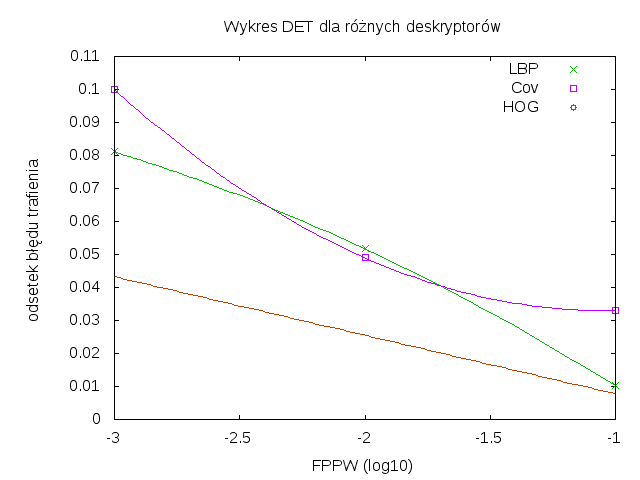
\includegraphics[width=0.8\textwidth]{joint_det.png}
\caption{Wspólny wykres DET dla przebadanych metod}
\label{fig:joint_det}
\end{figure}
\chapter{Łączenie działania deskryptorów}
\label{cha:laczenie}

\section{Wprowadzenie}
Biorąc pod uwagę to, że każdy z elementów wektora traktowany jest przez klasyfikator jako zmienna niezależna od reszty, połączenie wynikowych wektorów dwóch lub więcej metod powinno pozwolić na jeszcze dokładniejsze opisanie danego obiektu. Szczególną korzyść można odnieść w przypadku, gdy łączone ze sobą deskryptory dokonują ekstrakcji cech z oryginalnego obrazu stosując odmienne podejście, dzięki czemu w nowo powstałych wektorach nie ma powielonych redundantnych informacji. Oczywiście kosztem potencjalnego poprawienia skuteczności metody, oprócz konieczności wyliczenia kilku wektorów cech, jest zwiększenie wymiarowości wynikowego wektora cech, co ciągnie za sobą dłuższy czas treningu klasyfikatora i klasyfikacji.

W przebadanych metodach, zarówno HOG jak kowariancja cech, bazują na informacjach dotyczących krawędzi obrazu wejściowego. Odmienne podejście zastosowano w metodzie LBP, która dokonuje ekstrakcji informacji dotyczących tekstury na obrazie. Biorąc pod uwagę powyższe, przebadano zachowanie następujących połączeń deskryptorów: HOG i LBP oraz macierzy kowariancji cech i LBP.

\section{Łączenie deskryptora kowariancji i LBP}

\subsection{Wyniki pierwszej walidacji}

W tabeli \ref{tab:covlbp_first} zestawiono wyniki krzyżowej walidacji pierwszego klasyfikatora wytrenowanego 
próbkami uzyskanymi w wyniku połączenia deskryptorów cech, wykorzystującego macierz kowariancji oraz LBP. Dla porównania zestawiono te wyniki z wynikami uzyskanymi dla pojedynczych deskryptorów.

\begin{center}
    \begin{longtable}{ | p{5cm} | p{3cm} | p{3cm} | p{3cm} |}
    \caption{Wyniki pierwszej walidacji krzyżowej przy użyciu łączonego deskryptora wykorzystującego macierz kowariancji cech i LBP}
    \label{tab:covlbp_first}\\
    \hline
	Metoda & Kowariancja & LBP & Połączenie \\ \hline
    Długość wektora cech & 832 & 4096 & 4928 \\ \hline
    Liczba pozytywnych detekcji w pozytywnym zbiorze testowym & 593 & 531 & 601 \\ \hline
    Liczba negatywnych detekcji w pozytywnym zbiorze testowym & 33 & 95 & 25 \\ \hline
    Celność metody w pozytywnym zbiorze testowym & \textbf{94,73\%} & \textbf{84,82\%} & \textbf{96,01\%} \\ \hline
    Liczba pozytywnych detekcji w negatywnych zbiorze testowym & 30 & 20 & 21 \\ \hline
    Liczba negatywnych detekcji w negatywnym zbiorze testowym & 876 & 886 & 885 \\ \hline
    Celność metody w negatywnym zbiorze testowym & \textbf{96,69\%} & \textbf{97,79\%} & \textbf{97,68\%} \\ \hline
    
    \end{longtable}
\end{center}


\subsection{Wyniki drugiej walidacji}
W tabeli \ref{tab:covlbp_second} zestawiono wyniki krzyżowej walidacji drugiego klasyfikatora po dotrenowaniu pierwszego klasyfikatora fałszywymi pozytywnymi detekcjami, wykrytymi w zbiorze testowym. W celu zminimalizowania efektu "przetrenowania" klasyfikatora wzięto pod uwagę 25\% fałszywie pozytywnych detekcji wygenerowanych na zbiorze testowym. Dla porównania zestawiono te wyniki z wynikami uzyskanymi dla pojedynczych deskryptorów.

\begin{center}
    \begin{longtable}{ | p{5cm} | p{3cm} | p{3cm} | p{3cm} |}
    \caption{Wyniki drugiej walidacji krzyżowej przy użyciu łączonego deskryptora wykorzystującego macierz kowariancji cech i LBP}
    \label{tab:covlbp_second}\\
    \hline
	Metoda & Kowariancja & LBP & Połączenie \\ \hline
    Długość wektora cech & 832 & 4096 & 4928 \\ \hline
    Liczba pozytywnych detekcji w pozytywnym zbiorze testowym & 502 & 512 & 584 \\ \hline
    Liczba negatywnych detekcji w pozytywnym zbiorze testowym & 124 & 134 & 40 \\ \hline
    Celność metody w pozytywnym zbiorze testowym & \textbf{80,20\%} & \textbf{81,79\%} & \textbf{93,29\%} \\ \hline
    Liczba pozytywnych detekcji w negatywnych zbiorze testowym & 19 & 30 & 17 \\ \hline
    Liczba negatywnych detekcji w negatywnym zbiorze testowym & 887 & 876 & 889 \\ \hline
    Celność metody w negatywnym zbiorze testowym & \textbf{97,90\%} & \textbf{96,69\%} & \textbf{98,12\%} \\ \hline
    \end{longtable}
\end{center}


\subsection{Rozkłady błędów detekcji}

Wykres rozkładu błędu detekcji przy połączeniu deskryptorów HOG i LBP zaprezentowany został na rysunku \ref{fig:covlbp_det}. Na podstawie wykresu można zauważyć, że połączenie metod wyraźnie poprawia skuteczność działania metody dla takiego samego rzędu fałszywie pozytywnych detekcji na obrazie. 

\begin{figure}[htb]
\centering
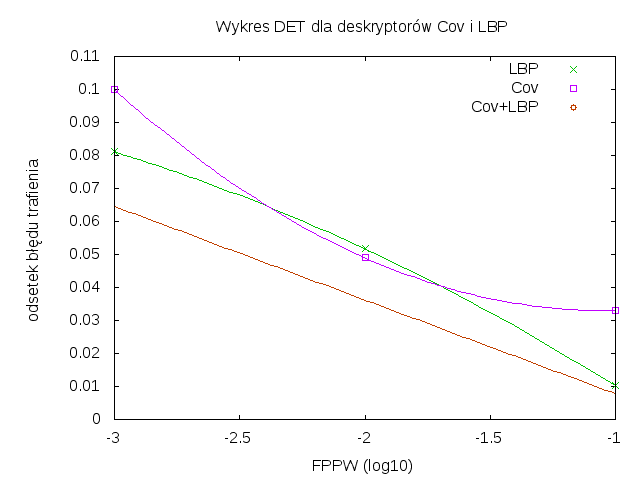
\includegraphics[width=0.9\textwidth]{covlbp_det.png}
\caption{Rozkład błędu detekcji dla połączenia metody LBP i kowariancji cech}
\label{fig:covlbp_det}
\end{figure}

\subsection{Analiza złożoności poszczególnych kroków metody}

W poniższej tabeli zestawiono czasy wykonywania poszczególnych kroków metodologii na konfiguracji testowej.
Dla porównania zestawiono te wyniki z wynikami uzyskanymi dla pojedynczych deskryptorów.

\begin{center}
    \begin{longtable}{ | p{5cm} | p{3cm} | p{3cm} | p{3cm} |}
    \hline
	Metoda & Kowariancja & LBP & Połączenie \\ \hline
    Ekstrakcja cech pozytywnych / próbka & 4,33 ms & 11,08 ms & 14,72 ms \\ \hline
    Ekstrakcja cech negatywnych / próbka & 3,54 ms & 10,19 ms & 13,86 ms\\ \hline
    Pierwszy trening klasyfikatora & 10,75 s & 27,67 s & 57,67 s \\ \hline
    Generacja fałszywie pozytywnych okien & 296,06 s & 657 s & 884,73 s \\ \hline
    Drugi trening klasyfikatora & 14,41 s & 31,62 s & 68,62 s \\ \hline
    Analiza rozkładu błędu detekcji w zbiorze testowym & 3172 s & 4914 s & 5200 s \\ \hline
    \caption{Czas wykonywania poszczególnych etapów badania przy użyciu łączonego deskryptora wykorzystującego macierz kowariancji cech i LBP} \\
    \end{longtable}
\end{center}

\subsection{Podsumowanie}

Nowo utworzony deskryptor można, pod względem jakościowym, ocenić znacznie lepiej niż jego pojedyncze składowe, używane do detekcji osobno. Potwierdza to zarówno rozkład DET porównany z~rozkładami dla składowych jak i wyniki krzyżowych walidacji, w szczególności po dotrenowaniu klasyfikatora. Odbywa się to jednak zwiększonym kosztem złożoności użycia nowej metody. Wynika to bezpośrednio z faktu, że klasyfikator operuje na znacznie większych wektorach cech, które powstają z połączenia dwóch.


\section{Łączenie deskryptora HOG i LBP}

\subsection{Wyniki pierwszej walidacji}

W poniższej tabeli zestawiono wyniki krzyżowej walidacji pierwszego klasyfikatora wytrenowanego 
próbkami uzyskanymi w wyniku połączenia deskryptorów cech, wykorzystującego deskryptory HOG oraz LBP. Dla porównania zestawiono te wyniki z wynikami uzyskanymi dla pojedynczych deskryptorów.

\begin{center}
    \begin{longtable}{ | p{5cm} | p{3cm} | p{3cm} | p{3cm} |}
    \hline
	Metoda & HOG & LBP & Połączenie \\ \hline
    Długość wektora cech & 7308 & 4096 & 11404 \\ \hline
    Liczba pozytywnych detekcji w pozytywnym zbiorze testowym & 575 & 531 & 585 \\ \hline
    Liczba negatywnych detekcji w pozytywnym zbiorze testowym & 57 & 95 & 41 \\ \hline
    Celność metody w pozytywnym zbiorze testowym & \textbf{91,85\%} & \textbf{84,82\%} & \textbf{93,45\%} \\ \hline
    Liczba pozytywnych detekcji w negatywnych zbiorze testowym & 31 & 20 & 21 \\ \hline
    Liczba negatywnych detekcji w negatywnym zbiorze testowym & 875 & 886 & 885 \\ \hline
    Celność metody w negatywnym zbiorze testowym & \textbf{96,58\%} & \textbf{97,79\%} & \textbf{97,68\%} \\ \hline
    \caption{Wyniki pierwszej walidacji krzyżowej przy użyciu łączonego deskryptora wykorzystującego deskryptory HOG i LBP} \\
    \end{longtable}
\end{center}


\subsection{Wyniki drugiej walidacji}
W poniższej tabeli zestawiono wyniki krzyżowej walidacji drugiego klasyfikatora po dotrenowaniu pierwszego klasyfikatora fałszywymi pozytywnymi detekcjami, wykrytymi w zbiorze testowym. W celu zminimalizowania efektu "przetrenowania" klasyfikatora wzięto pod uwagę 25\% fałszywie pozytywnych detekcji wygenerowanych na zbiorze testowym. Dla porównania zestawiono te wyniki z wynikami uzyskanymi dla pojedynczych deskryptorów.

\begin{center}
    \begin{longtable}{ | p{5cm} | p{3cm} | p{3cm} | p{3cm} |}
    \hline
	Metoda & HOG & LBP & Połączenie \\ \hline
    Długość wektora cech & 7308 & 4096 & 11404 \\ \hline
    Liczba pozytywnych detekcji w pozytywnym zbiorze testowym & 531 & 512 & 564 \\ \hline
    Liczba negatywnych detekcji w pozytywnym zbiorze testowym & 95 & 134 & 60 \\ \hline
    Celność metody w pozytywnym zbiorze testowym & \textbf{84,82\%} & \textbf{81,79\%} & \textbf{90,10\%} \\ \hline
    Liczba pozytywnych detekcji w negatywnych zbiorze testowym & 32 & 30 & 13 \\ \hline
    Liczba negatywnych detekcji w negatywnym zbiorze testowym & 874 & 876 & 893 \\ \hline
    Celność metody w negatywnym zbiorze testowym & \textbf{96,47\%} & \textbf{96,69\%} & \textbf{98,57\%} \\ \hline
    \caption{Wyniki drugiej walidacji krzyżowej przy użyciu łączonego deskryptora wykorzystującego deskryptory HOG i LBP} \\
    \end{longtable}
\end{center}


\subsection{Rozkłady błędów detekcji}

Wykres rozkładu błędu detekcji przy połączeniu deskryptorów HOG i LBP zaprezentowany został na rysunku \ref{fig:hoglbp_det}. Na podstawie wykresu można zauważyć, że połączenie tych metod nie poprawia działania klasyfikatora, a w kontekście zbioru testowego i metodologii, na którym został badany nawet nieco pogarsza.

\begin{figure}[htb]
\centering
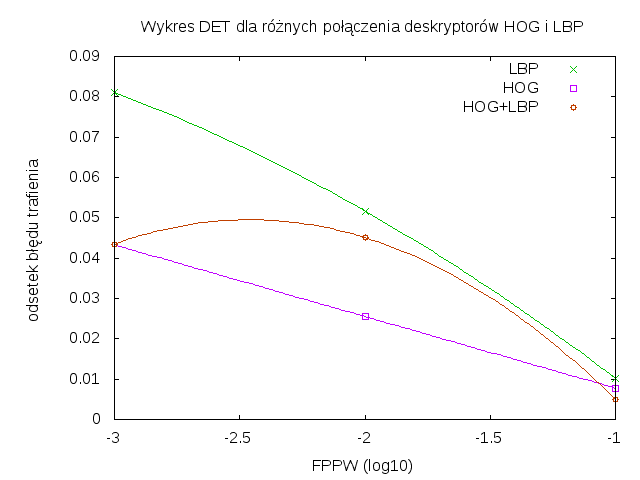
\includegraphics[width=0.9\textwidth]{hoglbp_det.png}
\caption{Rozkład błędu detekcji dla połączenia metody LBP iHOG}
\label{fig:hoglbp_det}
\end{figure}

\subsection{Analiza złożoności poszczególnych kroków metody}

W poniższej tabeli zestawiono czasy wykonywania poszczególnych kroków metodologii na konfiguracji testowej.
Dla porównania zestawiono te wyniki z wynikami uzyskanymi dla pojedynczych deskryptorów.

\begin{center}
    \begin{longtable}{ | p{5cm} | p{3cm} | p{3cm} | p{3cm} |}
    \hline
	Metoda & HOG & LBP & Połączenie \\ \hline
    Ekstrakcja cech pozytywnych / próbka & 6,23 ms & 11,08 ms & 15,24 ms \\ \hline
    Ekstrakcja cech negatywnych / próbka & 5,27 ms & 10,19 ms & 14,05 ms\\ \hline
    Pierwszy trening klasyfikatora & 33,69 s & 27,67 s & 69,89 s \\ \hline
    Generacja fałszywie pozytywnych okien & 590,40 s & 657 s & 987,32 s \\ \hline
    Drugi trening klasyfikatora & 40,62 s & 31,62 & 82,39 s \\ \hline
    Analiza rozkładu błędu detekcji w zbiorze testowym & 1938 s & 4914 s & 5730 s \\ \hline
    \caption{Czas wykonywania poszczególnych etapów badania przy użyciu łączonego deskryptora wykorzystującego macierz kowariancji cech i LBP} \\
    \end{longtable}
\end{center}

\subsection{Podsumowanie}
Biorąc pod uwagę wyniki walidacji krzyżowej, z której można wywnioskować nieznaczną poprawę działania deskryptora HOG, a także wykres rozkładu błędu detekcji, który sugeruje negatywny wpływ połączenia, można dojść do wniosku, że w kontekście detekcji sylwetek ludzkich deskryptor LBP w~słabym stopniu uzupełnia metodę HOG.
\chapter{Podsumowanie}
\label{cha:wnioski}

W niniejszej pracy przeprowadzono badania literatury naukowej pod kątem wybranych metod tworzenia deskryptorów cech używanych w metodach detekcji obiektów. Ponadto, zaprezentowano kompletną metodologię służącą do przebadania, zarówno pod kątem jakościowym jak i złożoności, danej metody - począwszy od generacji negatywnego zbioru testowego, przez ekstrakcję cech, budowę pierwszego i dotrenowanego klasyfikatora, walidacje klasyfikatora, aż po budowę rozkładu błędu detekcji, który jest pomocnym narzędziem przy wyborze metody detekcji do konkretnego zastosowania.

Korzystając z powyższej metodologii przebadano trzy z czterech przeanalizowanych metod i porównano je. Dokonano także próby przystosowania ostatniej z nich, metody \textit{edgelets} do metodologii, w~której do klasyfikacji używany jest mocny klasyfikator, jak SVM.

Oprócz tego przebadano, korzystając z tej samej metodologii, efekt połączenia ze sobą dwóch metod. Jak wynika z przeprowadzonych badań, łączenie działania deskryptorów pozwala na polepszenie skuteczności detekcji, gdy połączone deskryptory zawierają niepokrywające się ze sobą informacje oraz metody te nie są dedykowane konkretnemu zastosowaniu. Takie ulepszenie odbywa się jednak kosztem złożoności czasowej.

W dalszej pracy warto dokonać próby budowy metody, podobnej do metody \textit{edgelets}, jednak potrafiącej dobrze opisywać obraz wejściowy przy pomocy niezbyt długiego wektora cech.
Można również zastanowić się nad znalezieniem deskryptora bazującego na metodzie LBP, jednak posiadającego lepsze właściwości opisu orientacji i długości krawędzi na obrazie. Próby takiej dokonali autorzy pracy \cite{Zhao07}, jednak w bardziej wymagających testach metoda ta okazuje się zawodna, prawdopodobnie poprzez zbyt ogólny deskryptor.
W dalszej pracy warto również przeprowadzić badania prowadzące do możliwości optymalizacji zaprezentowanych metod i algorytmów pod kątem zrównoleglenia wykonywania poszczególnych operacji prowadzących do obliczenia wartości żądanego deskryptora cech. Zbadanie możliwości wykonywania części lub całości poszczególnych algorytmów na wielu rdzeniach jednocześnie pozwoli na zastanowienie się nad możliwością ich przyspieszenia w rzeczywistych zastosowaniach.



% itd.
% \appendix
% \include{dodatekA}
% \include{dodatekB}
% itd.

\bibliographystyle{alpha}
\bibliography{bibliografia}

\end{document}
